\documentclass[11pt, a4paper]{article}
\usepackage[nochapters]{classicthesis}                              % template
\usepackage[margin=42mm]{geometry}                                  % margins
\usepackage[utf8]{inputenc}                                         % allow utf-8 input
\usepackage[T1]{fontenc}                                            % use 8-bit T1 fonts
\usepackage{graphicx}                                               % images
\usepackage{url}                                                    % URL typesetting
\usepackage{booktabs}                                               % good-looking tables
\usepackage{multirow}                                               % for tables
\usepackage{amsfonts}                                               % blackboard math symbols
\usepackage{amsmath}                                                % math ops
\usepackage{nicefrac}                                               % compact 1/2, etc.
\usepackage{microtype}                                              % microtypography
\usepackage{float} %to force figures to appear at a specific location
\usepackage{subcaption}
\usepackage{tabularx}

\definecolor{darkblue}{rgb}{0, 0, 0.5}                              % define link color
\hypersetup{colorlinks=true,citecolor=darkblue,                     % set link color
            linkcolor=darkblue, urlcolor=darkblue}

% Your packages here
% \usepackage{...}                                                  % some info, maybe

% !!! PLEASE CHANGE THESE VARIABLES TO MATCH YOUR INFORMATION !!!

\def\thesistitle{Predicting Pilot Performance in VR Flight Training Using Tree-Based Multi-Output Regression}                      % title
\def\subtitle{}             % subtitle
    % ^if there is no subtitle, replace by \def\subtitle{}  
\def\yourname{Yijun Wu}                                                                       % ^first and last nam
 \def\yourprogramme{Cognitive Science \& Artificial Intelligence}    % uncomment this
\def\yourstudentnumber{2066623}                                      % ANR (or u-number)
\def\finalmonth{January}
\def\finalyear{2000}
\def\supervisor{dr. Phillip Brown}
\def\committee{dr. Silvia-Laura Pintea}
\def\acknowledgments{I would like to express my sincere gratitude to my supervisor, Dr. Phillip Brown, for his invaluable guidance, support, and encouragement throughout this research.}
\def\wordcount{7876}
% METADATA

\hypersetup{pdfauthor   = \yourname,
            pdftitle    = \thesistitle\ \subtitle,
            pdfsubject  = \yourprogramme\ Master Thesis
}

% CHOOSE EITHER OF -----------------------------------------
% IEEE STYLE:

\usepackage[square,numbers]{natbib}                               % bracket-style refs
\usepackage{natbib}                                               % OR: parenthesized refs
\bibliographystyle{IEEEtranN}

% OR -------------------

%\usepackage[natbibapa]{apacite}                                     % only parentheses
%\bibliographystyle{apacite}                                         % 'cause APA

% !!! ------------------------------------------------------ !!!

\begin{document}
\input{frontmatter.tex}  % don't remove this :)

% --- start writing below:

\begin{abstract}
This study examines how accurately pilot performance during a virtual reality ILS landing task can be predicted in near real time using tree-based machine learning models trained on multimodal physiological and simulator-derived features. The goal is to assess whether such models can support automated, continuous monitoring in pilot training. Analyses use the CogPilot dataset, which contains synchronized ECG, respiration, and aircraft-behavior data. Heart-rate and respiration features were extracted from sliding 10-second windows and combined with aircraft state variables to form second-by-second observations. Three tree-based multi-output regressors were trained to predict four continuous performance-error labels (glide slope, localizer, airspeed, and total tracking error) and were evaluated using two generalization strategies. Models achieved high predictive accuracy when the feature set included lagged component error inputs, whereas they yielded only modest but non-negligible performance when limited to physiological and simulator-derived features. These findings indicate that tree-based regression models can underpin automated, short-horizon performance monitoring in VR-based pilot training, while physiology-driven models are particularly relevant when recent performance data are unavailable, delayed, or noisy.
\end{abstract}

\section{Data Source, Ethics, Code, and Technology statement}
Data Source:
The data used in this thesis come from the publicly available CogPilot dataset, published on PhysioNet \cite{goldberger-2000} by \cite{rao-2022}, who remain the owners of the data. No new data were collected for this project, and the research did not involve direct interaction with human participants or animals. The dataset is anonymized and was obtained through an online request and download from the PhysioNet repository in accordance with its terms of use.

Code:
All preprocessing, modeling, and analysis code was written by the author in Python, using the libraries NeuroKit2, pandas, NumPy, scikit‑learn, XGBoost, CatBoost, Matplotlib, and seaborn. The thesis code can be accessed through the GitHub repository following the link \href{https://github.com/Yijun-cat/Bachelor_Thesis_Project.git}{https://github.com/Yijun-cat/Bachelor\_Thesis\_Project.git}. Where code patterns followed standard examples from package documentation or tutorials, these were adapted and integrated into the author’s own pipelines; this work did not make direct use of proprietary or unpublished code developed in prior research.

Figures:
All figures in this thesis were generated by the author using the analysis code developed for this project, based on the dataset and derived model outputs. All images and figures in this work were created specifically for this study.

Technology:
During the preparation of this work, the author used Perplexity \cite{perplexity-ai-2026}, powered by GPT‑5.1 \cite{openai-2025}, in order to assist with brainstorming, language polishing, and checking the clarity and consistency of the manuscript text. After using this tool, the author reviewed and edited the content as needed and takes full responsibility for the final text of the thesis. Standard spelling and grammar checking tools integrated in the word processing and LaTeX environment were also used. No additional tools or services were used for typesetting beyond the official Tilburg University LaTeX template and its associated reference management workflow.

\section{Introduction} \label{sec:introduction}
High‑stakes professional training involves learning complex motor and cognitive skills, while strict safety regulations and restricted training resources make attaining expert competency difficult \cite{nassar-2021}. In the aviation industry, pilot training plays a vital role and is directly linked to both flight safety and the effective execution of flight operations \cite{yang-2021}. However, the current training framework is largely instructor‑led and can lead to high instructor workload, subjective trainee evaluation, and a lack of real‑time feedback on risky behaviors \cite{yang-2021}. Multiple studies have examined the use of machine learning (ML) methods in combination with virtual reality (VR) to address these challenges; nevertheless, the adoption of ML in pilot training and education remains comparatively limited \cite{caballero-2023}. In such adaptive training systems, ML-based models are used to estimate trainee performance and state from behavior and physiological data \cite{madrigal-cerezo-2026}. These estimates provide the information needed to adjust task difficulty and feedback in real time, enabling individualized and responsive training \cite{madrigal-cerezo-2026}. Moreover, ML approaches that leverage physiological signals from trainee pilots can be integrated into legacy training equipment and simulators \cite{caballero-2023}, and they enable more precise and continuous error measurement, reducing the need for labor‑intensive evaluations by human instructors \cite{barry-2025}. Building on these developments, the present project investigates near real‑time task performance prediction with ML models that are trained on multimodal physiological and simulator‑derived data, with the aim of guiding the design of adaptive and scalable pilot training systems.

This thesis advances research on physiology-based flight performance modeling by systematically assessing tree‑based regression methods for the continuous prediction of multiple performance-error metrics in a VR landing task. Psychophysiological signals have been used in prior work to monitor pilot performance in real time and to forecast fatigue \cite{alreshidi-2024,dideriksen-2019,wilson-2019}, demonstrating the feasibility of physiology‑informed performance models in aviation contexts. Many of these studies, however, have focused on either physical cockpits with $2$D simulator displays or real‑flight scenarios, and performance monitoring and modeling in fully immersive VR training contexts have received comparatively less attention. Existing work in VR‑integrated simulators has often relied on single‑modal physiological inputs when applying machine learning to analysis of pilot performance \cite{moore-2023,rajendran-2021}. Because adaptive training systems adjust task difficulty and workload based on ongoing assessments of trainee performance \cite{fraulini-2024}, accurate and near real-time performance models are critical for their design. From a scientific perspective, by analysing how multimodal physiological and simulator-derived features can support second-by-second prediction of flight path errors in VR landings, this thesis provides empirical evidence for the performance modeling component required to design such adaptive systems.

Growing worries about flight safety, limited availability of skilled pilots and instructors, and the swift technological evolution of the aviation sector have made flight simulators increasingly important for training and research \cite{wang-2024}. Virtual reality has enhanced simulator‑based pilot training by adding VR headsets to existing systems and delivering high‑fidelity $3$D flight scenarios, creating immersive, realistic virtual cockpits while also improving cost‑effectiveness, safety, and training efficiency \cite{wang-2024}. Despite these advantages, current simulator-based training still depends extensively on human instructors and evaluators for continuous performance monitoring and adaptive difficulty adjustment, which constrains training output when instructor resources are limited \cite{caballero-2023}. Adaptive automated training systems that continuously monitor pilot performance and dynamically adjust task difficulty could help alleviate these constraints and reduce the operational burden on active pilots who serve as instructors \cite{barry-2025}. VR is well suited for such adaptive training systems because it provides immersive, controllable training scenarios and detailed simulator and sensor data that can be used to monitor performance continuously \cite{reyes-2022}. From a societal perspective, by enabling more accurate and timely prediction of task performance from multimodal physiological and simulator-derived data, the models examined in this thesis can guide the design of such systems and support safer and more scalable pilot training.

The central research question of this thesis is therefore:

\begin{quote}
\emph{How accurately can task performance during virtual reality pilot training tasks be predicted in near real time using tree‑based machine learning models trained on multimodal physiological and simulator‑derived features?}
\end{quote}

%\noindent The sub-questions can be listed seperately, as such:
This overarching question is addressed through the following sub-questions:
\begin{itemize}
    \item[RQ1] \emph{To what extent does adding short-term performance history (lagged error features) improve predictive accuracy compared to using only physiological and simulator-derived inputs?}
    \item[RQ2] \emph{Which input features (physiological, simulator-derived, and lagged error features) contribute most to prediction performance in the trained models?}
\end{itemize}

The research question is addressed by training three tree-based regression models (Random Forest, XGBoost, and CatBoost), which are well suited to modeling nonlinear relationships in structured tabular data with mixed feature types \cite{grinsztajn-2022,uddin-2024}, to generate per‑second predictions of error measurements (glide slope, localizer, airspeed, and total error) during VR landing tasks from electrocardiography- and respiration-derived features together with simulator variables. Models using only physiological and aircraft features achieve low predictive accuracy, whereas including online computed one- and two-second lagged error measurements as additional inputs yields substantial improvements in all evaluation metrics. These findings indicate that tree-based models with simple lagged inputs can support accurate, near real-time monitoring of performance errors in an adaptive VR-based pilot training simulator, provided that recent task performance is continuously recorded.

\section{Related Work}
This section reviews prior work relevant to VR pilot training, physiological measurement, and machine learning-based performance modeling. The aim is to position the present study within the broader literature and to highlight how existing approaches inform, but also differ from the goals of this thesis.

\subsection{VR in Aviation Training}
Virtual reality (VR) has increasingly been adopted across multiple domains of aviation training, ranging from initial pilot training for beginners to aircraft maintenance and service roles \cite{fussell-2020,hight-2022,pena-2025}. Studies with student pilots have evaluated VR flight simulators as primary or supplementary training devices and typically compare them to desktop‑based or traditional aviation training devices \cite{hight-2022,guthridge-2023}. These developments highlight its potential as a general-purpose medium for high-fidelity simulation in aviation.

The effectiveness of VR in pilot training has been assessed in a number of empirical studies. For basic flight training, Hight \emph{et al.} \cite{hight-2022} conducted a quasi‑experimental pilot study with civilian pilots, comparing desktop $2$D simulations and head‑mounted VR simulations while keeping other training factors identical. They found no significant differences in academic performance between the VR and $2$D conditions, based on module and final scores, and also collected subjective ratings of the learning materials. Their findings suggest that VR does not hinder skill acquisition, and that students in both conditions rated simulation‑based training as highly beneficial and preferred it over other learning media \cite{hight-2022}. In another study, Guthridge and Clinton‑Lisell \cite{guthridge-2023} evaluated beginning-level instrument pilots' pretest and post-test performance on a visual traffic pattern task after trained in either VR simulator, a PC-based simulator, or no simulator. The findings indicated that participants in both the VR and PC‑based training conditions showed significant improvement in flight maneuvers relative to the group without simulator training, with the VR group performing broadly comparably to the PC‑based group \cite{guthridge-2023}. Students also perceived VR as an acceptable and immersive training technology \cite{guthridge-2023}. Van Weelden \emph{et al.} \cite{van-weelden-2024} examined differences in EEG-based workload and flight performance between 2D desktop and 3D VR versions of a PC-7 flight simulator. In a within-subjects design, participants without prior flight experience completed two maneuvering tasks in both display conditions. The study found that the VR condition elicited higher task engagement and improved training performance.

These studies suggest that immersive VR simulators can support training outcomes comparable to those achieved with $2$D desktop or PC‑based simulators. Students generally perceive both $2$D and VR simulations as beneficial and often prefer simulator‑based practice over more traditional learning materials \cite{hight-2022,guthridge-2023}, even though current VR systems still present technical, implementation, and integration challenges \cite{pena-2025}. However, existing evaluation methods mostly rely on aggregated academic performance or discrete measures of maneuver accuracy rather than continuous, time‑resolved performance metrics or physiology‑informed models. This methodological emphasis underscores a persisting gap in the literature and motivates the present thesis, which seeks to integrate VR flight tasks with multimodal physiological monitoring and machine‑learning‑based performance prediction.

\subsection{Physiological Measures of Workload in Pilot Training}
A number of studies have investigated how ECG‑ and respiration‑based measures reflect cognitive load and stress in simulated flight tasks. Korner \emph{et al.} \cite{koerner-2025} examined heart rate as an index of mental workload and performance in VR landing tasks, found that mean heart rate climbed as tasks became harder, gradually fell across repeated runs at a given difficulty, and peaked near touchdown relative to the onset of the flight, while showing a positive association with subjective workload and a negative association with performance. These results indicate that heart rate can support real‑time task‑difficulty adaptation to ensure that trainees remain in a target workload zone \cite{koerner-2025}. Bruna \emph{et al.} \cite{bruna-2018} investigated ECG and respiration during simulated emergency landings and related them to pilots’ subjective stress ratings, and reported that ECG‑derived heart‑rate variability parameters showed no significant changes across flight phases, whereas several respiration features, including average breathing frequency and low‑frequency respiratory power, increased during approach and landing \cite{bruna-2018}. These findings suggest that breathing rate and spectral power are sensitive markers of elevated workload and stress in high‑demand piloting scenarios \cite{bruna-2018}.

While these studies demonstrate that physiological data provide useful indicators of mental workload and stress, they primarily focus on analyses of physiology averaged over discrete flight phases or conditions and treat physiology as an outcome or indicator of task demand rather than as input to models predicting continuous performance. In contrast, the present thesis incorporates ECG‑ and respiration‑derived features, together with simulator‑derived variables, into tree‑based regression models that aim to predict performance errors in near real time. By evaluating how well these models generalize across subjects and over future time segments within runs, the thesis investigates the extent to which multimodal physiological signals can support continuous, sample‑wise prediction of pilot performance.

\subsection{Machine Learning for VR Flight Performance Prediction}
Previous research has examined the use of machine learning models trained on different physiological and simulator‑derived signals to support the development of adaptive VR‑integrated flight simulators for pilot training. A widely adopted dataset in this context is the CogPilot \cite{rao-2022} corpus, which provides multimodal physiological measurements together with simulator data from participants engaged in virtual‑reality landing maneuvers. Caballero \emph{et al.} \cite{caballero-2023} used this dataset to classify flight difficulty from multimodal physiological signals, training an AdaBoost‑based pipeline on features derived via functional principal component analysis and feature selection, and achieving around 87\% accuracy with an Area Under the Curve (AUC) of 0.88. Building on the same dataset, Moore \emph{et al.} \cite{moore-2023} addressed the same classification task using eye‑tracking and electrodermal activity signals, combining the Minimally Random Convolutional Kernel Transform with a deep neural network; the model reached an AUC of 0.91 and compressed the time‑series input by about 99.7\%. More recently, Barry \emph{et al.} \cite{barry-2025} proposed a multi-modal functional learning framework for landing‑error regression on the same dataset, transforming high‑frequency physiological and aircraft signals into tabular features using summary statistics and functional principal component analysis, applying feature selection with BorutaSHAP, and training several tree‑based models to predict approach‑error metrics.

Together, these studies demonstrate that multimodal time‑series from VR flight tasks can be effectively leveraged by machine learning models for both flight‑difficulty classification and offline prediction of landing performance, and they provide an important methodological foundation for intelligent instructor and evaluator systems. However, existing work predominantly targets post‑hoc analysis using either discrete difficulty labels or aggregated performance scores, and does not address continuous, near real‑time prediction of approach‑error trajectories or systematically examine subject‑level and temporal generalization behavior of different tree‑based model families. The present thesis extends this line of research by applying and comparing tree‑based multi‑output regression models to predict performance metrics in near real time from multimodal physiological and simulator‑derived features, and by explicitly analyzing their generalization across unseen pilots and across future time segments within runs.


\section{Methods}
The following sections provide an overview of the dataset, the extraction of physiological and aircraft features in sliding time windows, and the construction of multi‑output targets. They also provide a brief summary of the machine learning model training and the metrics used for evaluation.

\subsection{Dataset}
The CogPilot \cite{rao-2022} dataset was used in this project and is publicly available via PhysioNet \cite{goldberger-2000}. The dataset contains multimodal physiological, task performance, and interaction data collected from 35 participants who each performed flight–landing tasks at various difficulty levels. In a virtual reality environment, each participant followed an Instrument Landing System (ILS) approach and primarily relied on cockpit instrument readings to land an aircraft along a prescribed ideal flight path \cite{rao-2022}. Each experimental session consisted of 3 blocks with 4 missions per block, resulting in 12 missions per participant, with one difficulty level per mission \cite{rao-2022}. A Summary of the overall difficulty structure is presented in Table~\ref{tab:task_level}.

\begin{table}[htbp]
	\caption{Overall task difficulty structure}
	\label{tab:task_level}
	\centering
	\small
	\begin{tabular}{llll}
		\toprule                                 	
		Difficulty      &Wind         &Visibility    &Turbulence \\ 
		\midrule
		1					&None			&Unlimited		&None \\
		\midrule
		2					&40\(^{\circ}\)(10 kts)  & 5 statue miles	&None \\
		\midrule
		\multirow{2}{*}{3}	&3000':80\(^{\circ}\)(10 kts)  & 3 statue miles & Light above 1000'\\
							&1000':140\(^{\circ}\)(10 kts) & 				& \\
		\midrule
		\multirow{3}{*}{4}	&4800':250\(^{\circ}\)(10 kts) &   &  \\
							&2800':80\(^{\circ}\)(15-20 kts) & 1 statue mile	& Light \\
							&800':200\(^{\circ}\)(15 kts)	&				& \\
		\bottomrule
	\end{tabular}
\end{table}

Multiple wearable sensors were used to record seven physiological modalities, with nominal sampling frequencies between 128 and 1024 Hz \cite{rao-2022}. These modalities comprise electromyography (EMG), accelerometry (ACC), electrodermal activity (EDA), electrocardiography (ECG), respiration (RESP), eye tracking (ETK), and photoplethysmography (PPG). A detailed overview of the functional data derived from each physiological signal is provided in Table~\ref{tab:multimodal} in Appendix A. Mission difficulty was manipulated via four distinct weather conditions \cite{rao-2022}. According to the dataset description, flight performance measures were derived and recorded in real time from the simulated aircraft state signals and grouped into three components, each ranging from -3 to 3 \cite{rao-2022}. A detailed description of the performance-error components and their value ranges is provided in Table~\ref{tab:error}.

\begin{table}[htbp]
	\caption{Overview of performance errors}
	\label{tab:error}
	\centering
	\small
	\begin{tabular}{llp{3cm}l}
		\toprule                                 	
		Variable      &Sampling Rate         &Description    &Range \\ 
		\midrule
		Localizer error		& 4 Hz	& Horizontal deviation from the center of the runway  & $[-3, 3]$ \\
		\midrule
		Glide slope error	& 4 Hz	& Vertical deviation from the ideal decent to the runway  & $[-3, 3]$ \\
		\midrule
		Airspeed error	& 4 Hz	& Deviation from the ideal speed  & $[-3, 3]$ \\
		\midrule
		Total error		& $-$		& Instantaneous sum of the localizer, glide slope, and airspeed errors  & $[-9, 9]$ \\
		\bottomrule
	\end{tabular}
\end{table}


\subsection{Feature Engineering}
Recordings of ECG and RESP were selected as the physiological modalities for feature preprocessing and extraction. Heart rate (HR) derived from ECG can be employed as a useful indicator for dynamically tuning task difficulty so that trainees remain in an optimal workload zone \cite{koerner-2025}, and respiratory behavior is a robust marker of cognitive processing, with mentally demanding tasks typically associated with an increased breathing rate (BR) and higher‑frequency ventilation \cite{grassmann-2016}.

The raw ECG signal was first processed with a Butterworth band‑pass filter covering the 8 to 20 Hz frequency range, as this passband has been shown to be optimal for QRS complex detection with a favorable ratio of signal to noise \cite{elgendi-2010}. R‑peaks were then detected in the cleaned signal using the QRS detection algorithm proposed by Elgendi \emph{et al.} \cite{elgendi-2010}. Subsequently, the signal‑quality index (SQI) mechanism from Zhao and Zhang \cite{zhao-2018} was applied to identify low‑quality ECG segments, and HR was computed from the detected R‑peaks only for 25 subjects with ECG recordings classified as having excellent quality (see Table~\ref{tab:dataset} for a summary of the dataset structure).

\begin{table}[htbp]
	\caption{Overview of the preprocessed dataset structure}
	\label{tab:dataset}
	\centering
	\small
	\begin{tabular}{ccc}
		\toprule                                 	
		Measure                        & Task difficulty        		&  Value      \\ 
		\midrule
		\multirow{4}{*}{Samples per run}  	&  1       & 356\textpm27 \\
											&  2    	& 389\textpm28 \\
											&  3     	& 382\textpm66   \\
											&  4		& 382\textpm65 \\
		\midrule
		\multirow{4}{*}{Samples per subject}  	&  1       & 1068\textpm58 \\
												&  2    	& 1168\textpm54 \\
												&  3     	& 1146\textpm90   \\
												&  4		& 1146\textpm145 \\
		\midrule
		\multirow{4}{*}{Minutes per run}  	&  1       & 5.94\textpm0.46 \\
											&  2    	& 6.50\textpm0.47 \\
											&  3     	& 6.40\textpm1.11   \\
											&  4		& 6.40\textpm1.07 \\
		\bottomrule
	\end{tabular}
\end{table}

For the RESP signals, an optimized breath detection algorithm developed by Khodadad \emph{et al.} \cite{khodadad-2018} was used to preprocess the respiratory traces and to derive breathing rate and respiratory peaks. This method has been shown to outperform conventional algorithms on breath detection in terms of receiver–operating–characteristic performance \cite{khodadad-2018}. Respiratory amplitude was computed as the difference between each respiratory peak and its preceding trough. 

For each subject, difficulty level, and run number, physiological and aircraft features were extracted using a sliding 10‑second window aligned to the performance timestamps. First, the performance, ECG, RESP, and aircraft data streams were converted from MATLAB time format to seconds and then aligned to a common time axis shared by all signals. A sliding window of length 10 seconds, spanning $(t-10$, $t]$, was then moved along the aligned performance timeline in steps of 1 second (see Figure~\ref{fig:sliding_window}). For each window, the last available performance sample within $(t-10$, $t]$ was used to assign the glide slope, localizer, airspeed, and total error as target variables at time $t$. 

\begin{figure}[htbp]
	\centering
	
\includegraphics[width=\textwidth]{sliding_window.png}
	\caption{Illustration of the sliding 10-second window} 
	\label{fig:sliding_window}
\end{figure}

Within the same 10‑second interval, time‑domain features were computed from the corresponding segments of the cleaned HR and respiration signals. In parallel, the mean aircraft elevation trim (nose-up/nose-down tendency of the aircraft), aileron trim  (adjustments of the aircraft’s roll), and landing‑gear position were computed over the window. Each 10‑second window thus yielded a single feature vector, comprising physiological and aircraft features summarizing the past 10 s, paired with the contemporaneous performance errors at time $t$.

\subsection{Machine Learning Setup}
All predictive analyses were conducted on the dataset constructed from the 10‑second windows described above. For each subject, difficulty level, and run number, physiological, aircraft, and performance information were aggregated into a feature matrix and a multi‑output target matrix, where each row represents one 10‑second window and the targets correspond to glide slope, localizer, airspeed, and total error at the end of the window. Two feature configurations were considered. In the without‑lagged‑features condition, the feature set contained only physiological and aircraft features derived from the current 10‑second window. In the with‑lagged‑features condition, the feature set was augmented with the 3 component performance‑error (localizer, glide slope, and airspeed) variables sampled at times $t-1$ and $t-2$ s, i.e., one and two seconds before the target time $t$. Thus, each row’s lagged features represent the most recent 1$-$2 seconds of performance history preceding the target point. In both feature configurations, the prediction targets were identical (see Figure~\ref{fig:feature_target} for an illustration of the ML pipeline).

\begin{figure}[htbp]
	\centering
	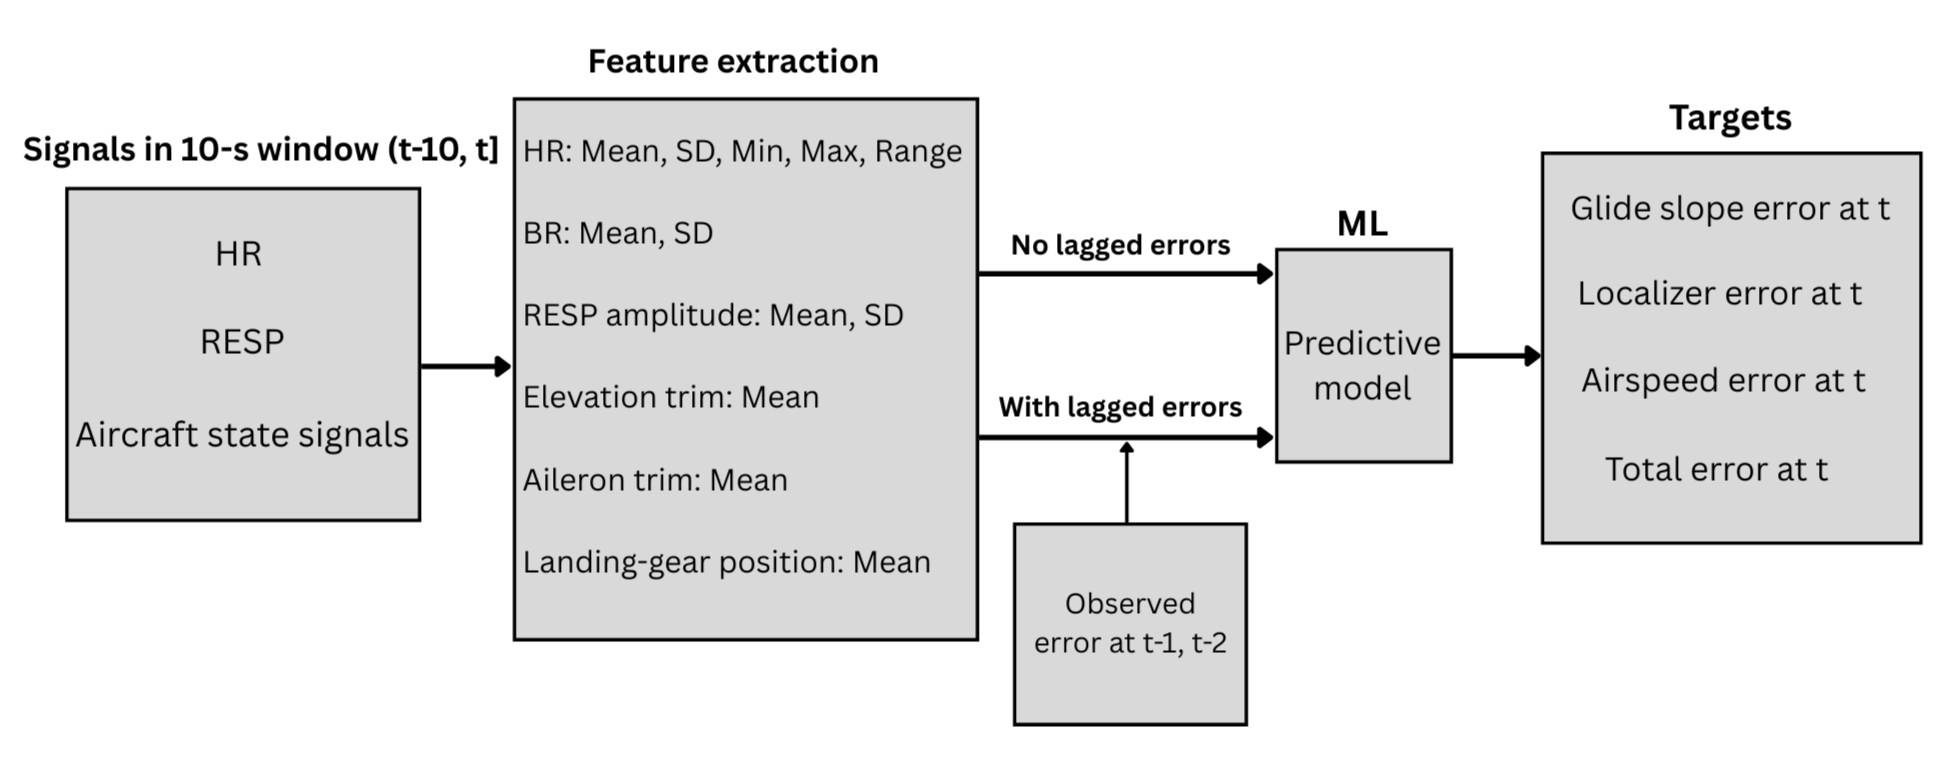
\includegraphics[width=\textwidth]{feature_vector.png}
	\caption{Machine‑Learning pipeline: feature extraction and prediction of error} 
	\label{fig:feature_target}
\end{figure}

To quantify how well the models generalize, two evaluation schemes were used that respect the hierarchical and temporal structure of the data. First, to assess generalization to new individuals, a leave‑one‑subject‑out (LOSO) cross‑validation procedure was employed, using the subject identifier as a grouping variable: in each fold, all windows from one participant were held out as test data and the models were trained on data from all remaining participants. Second, to assess generalization forward in time within the same runs, the last 60 s were held out as a test segment to evaluate whether models trained on earlier parts of the run could predict performance during the final, most demanding part of the landing task. The same 10-second sliding window procedure described above was applied within each 60-second test segment, yielding per-second predictions for times from 10 to 60 s. On the remaining data, grouped 5‑fold cross‑validation was used, with groups defined as unique subject–run combinations so that all windows from a given run were always assigned to the same fold. In both evaluation schemes, hyperparameters were tuned only on the training-validation data within the corresponding cross-validation procedure, and the chosen configuration was then refitted on the full training-validation set before testing on the held-out subject or the held-out 60-second segments. Figures~\ref{fig:loso} and \ref{fig:gkf} demonstrate the two generalization strategies.

\begin{figure}[htbp]
	\centering
	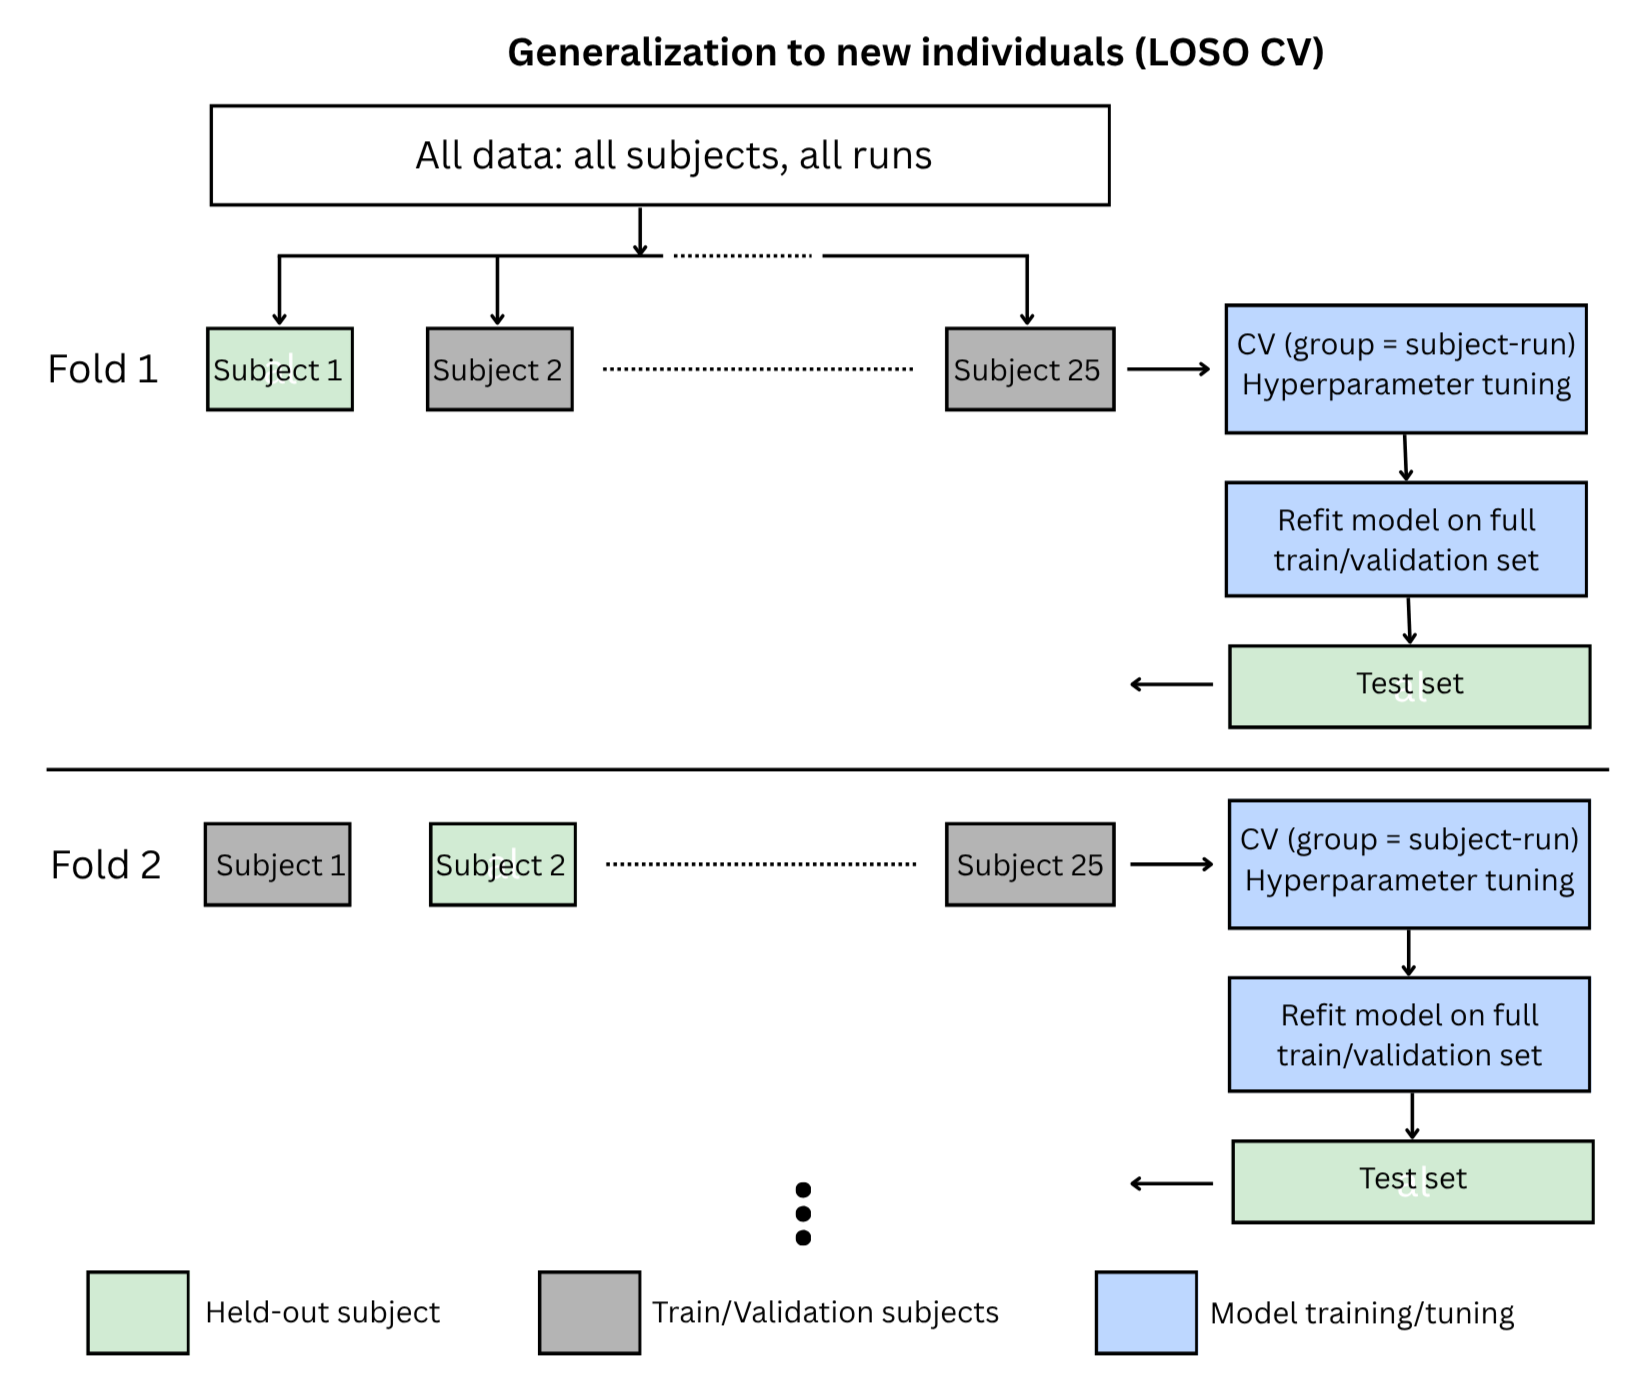
\includegraphics[width=\textwidth]{loso.png}
	\caption{Generalization to unseen individuals} 
	\label{fig:loso}
\end{figure}

\begin{figure}[htbp]
	\centering
	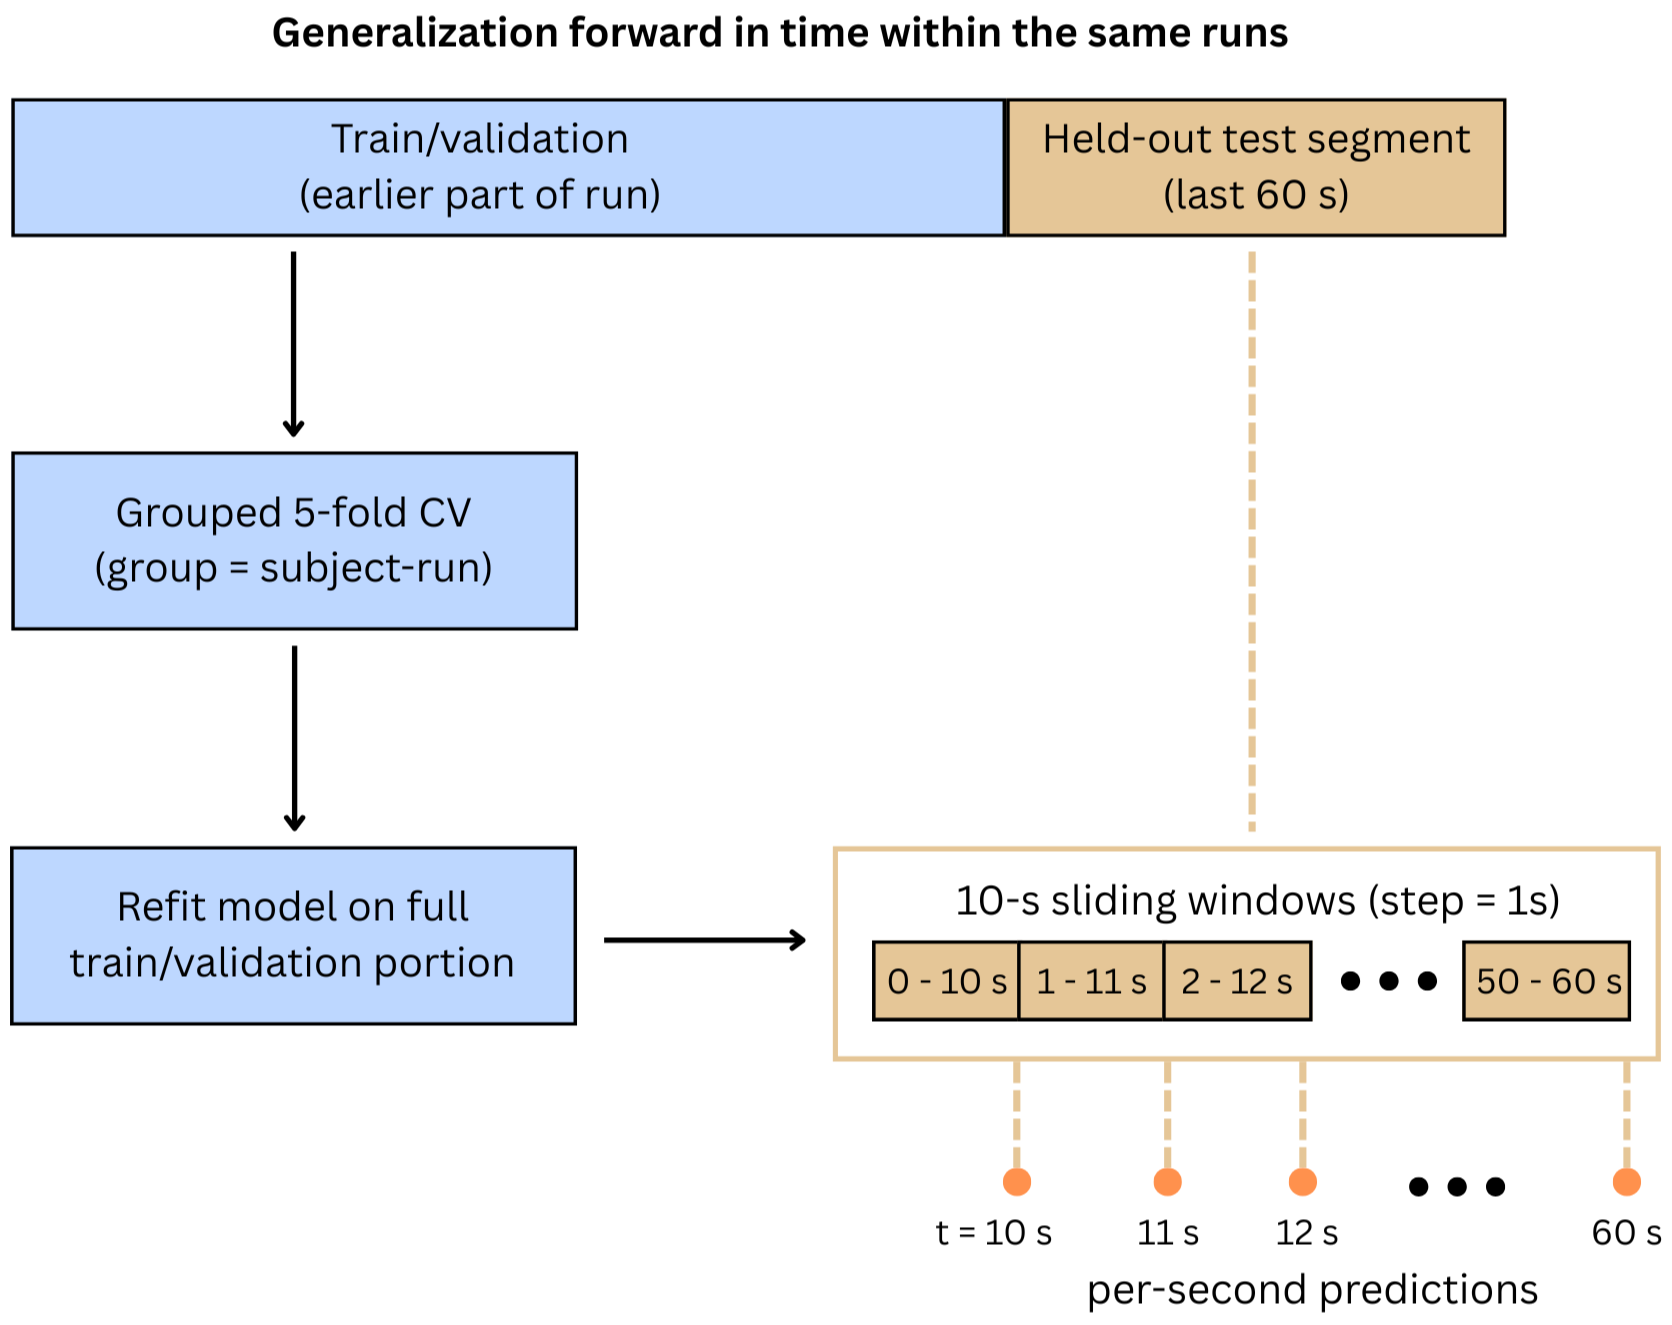
\includegraphics[width=\textwidth]{gkf.png}
	\caption{Generalization to the last 60s in the same run} 
	\label{fig:gkf}
\end{figure}

Three tree‑based regression algorithms were used for model training and evaluation: Random Forest (RF), XGBoost (XGB), and CatBoost (CB). Barry \emph{et al.} \cite{barry-2025} implemented the same models on this dataset using a post‑hoc approach to predict performance error, and observed that tree-based ensemble regressors are capable of capturing the majority of predictable variance in this task with relatively modest model complexity. Building on this evidence, the present study extends this work by systematically examining real‑time forecasting performance across feature configurations (including lagged error vs excluding lagged error) and generalization strategies. For each algorithm, a discrete hyperparameter grid was specified to reflect key design choices, and hyperparameter optimization was performed using exhaustive grid search with cross‑validation. The negative root mean squared error, averaged across output variables, served as the selection criterion for the best estimator. The explored hyperparameters and their candidate values are summarized in Table~\ref{tab:hyperparam}.

\begin{table}[htbp]
	\caption{Candidate model hyperparameters}
	\label{tab:hyperparam}
	\centering
	\small
	\begin{tabular}{lll}
		\toprule                                 	
		Model                        &  Hyperparameter        		&  Values      \\ 
		\midrule
		\multirow{4}{*}{Random Forest}  & Number of Estimators         	& [50, 100, 150] \\
										& Minimum Samples per Split    	& [2, 3, 4] \\
										& Minimum Samples per Leaf     	& [2, 3, 4]   \\
										& Bootstrapping					& [True, False] \\
		\midrule
		\multirow{3}{*}{XGBoost}  		& Number of Estimators          & [10, 100]      \\
										& Maximum Depth   				& [2, 3, 4, 5]    \\
										& Columns Sampled by Tree       & [0.3, 0.4, 0.5]  \\
		\midrule
		\multirow{3}{*}{CatBoost}       & Maximum Depth          		& [2, 3] \\
										& Learning Rate					& [0.01, 0.02, 0.03, 0.05]\\
                               			& L2 Regularization Coefficient	& [6, 10] \\
		\bottomrule
	\end{tabular}
\end{table}

\subsection{Evaluation Metrics}
Model performance was evaluated using root mean squared error (RMSE), mean absolute error (MAE), and the coefficient of determination R$^2$. RMSE quantifies prediction error in the same units as the target variables and places greater weight on larger errors \cite{barry-2025}, whereas MAE provides a complementary, more robust measure of typical error magnitude that is less sensitive to outliers. R$^2$ captures the proportion of variance in each target explained by the model and serves as the primary indicator of overall model fit. For each cross‑validation setting, the mean and standard deviation of these metrics across folds are reported, along with an overall mean aggregated across targets.

Furthermore, to assess whether the models preserved the relationships between specific error components and overall performance, Pearson correlations between component errors (glide slope, localizer, airspeed) and total error were examined for both true values and model predictions. These correlations were computed across all test samples within each evaluation setting and are reported alongside the primary error metrics.

\subsection{Implementation}
All preprocessing, modeling, and analysis code was implemented in Python using NeuroKit2, pandas, NumPy, and scikit-learn for data handling and the baseline model, XGBoost and Catboost for gradient boosting models, and Matplotlab/seaborn for visualization. Model explainability was examined using SHapley Additive exPlanations (SHAP) to inspect feature contributions for selected outputs. For each final model, SHAP values were computed on a subsample of 1,000 time points, and summary plots as well as local waterfall plots were generated to identify which features most strongly influenced the predicted performance errors.

\section{Results}\label{sec:results}
This section reports the performance of three tree-based models for task performance prediction. First, the extent to which the models generalize to new individuals and to later time points within the same trial is summarized. Next, error correlations and feature importance are examined.

\subsection{Generalization to new individuals}
This section evaluates how well the three models generalize to unseen subjects, first by comparing mean performance across subjects and error outputs, and then by examining individual error types and per-subject variability.

Table~\ref{tab:sub-overall} presents the mean MAE, RMSE, and R$^2$ across all error outputs and subjects for the Random Forest baseline, XGBoost, and CatBoost, either excluding or including lagged component errors as input features. In the first condition (without lagged errors), all models yield negative overall R$^2$ values, indicating that, on average, they perform worse than a simple mean predictor, with Random Forest showing the poorest fit. In the second condition, when the recent history of component errors is included as input, overall R$^2$ rises to approximately 0.96 for Random Forest and XGBoost and to 0.97 for CatBoost, accompanied by substantial reductions in MAE and RMSE.


\begin{table}[htbp]
	\caption{Model performance on held-out subjects}
	\label{tab:sub-overall}
	\centering
	\small
	\begin{tabular}{p{3cm}llll}
		\toprule                                 	
		Input Condition 	&Model          	&  Mean MAE      &  Mean RMSE      & Mean R$^2$ \\ 
		\midrule
		\multirow{3}{*}{No lagged errors} &RF  & 0.71 & 0.97 & -1.21 \\
														&XGB & 0.69  	& 0.92  & -0.83 \\
														&CB   & 0.67  & 0.89 & -0.68 \\
		\midrule
		\multirow{3}{*}{With lagged errors} &RF   & 0.07 	& 0.13 & 0.96 \\
														&XGB         & 0.07 & 0.12 & 0.96 \\
														&CB  & 0.06 	& 0.10 & 0.97\\ 
		\bottomrule
	\end{tabular}
\end{table}

 Table~\ref{tab:per-output-cb} shows per‑output performance for the CatBoost model. For glide slope and localizer errors, R$^2$ values of approximately 0.98 indicate that the model captures most of the between‑subject variance in these outcomes, whereas airspeed and total error show slightly lower but still high explained variance (R$^2$ $\approx$ 0.96). The corresponding Figure~\ref{fig:scatter-all} in Appendix A shows that predicted values cluster tightly around the identity line for all outputs, indicating that both the direction and magnitude of subject‑level deviations are reproduced well. 

\begin{table}[htbp]
	\caption{Per-output performance for CatBoost on held-out subjects}
	\label{tab:per-output-cb}
	\centering
	\small
	\begin{tabular}{lccc}
		\toprule                                 	
		Output          	& MAE      & RMSE      & R$^2$ \\ 
		\midrule
		Glide slope 	& 0.03\textpm0.01  	& 0.07\textpm0.05  & 0.98\textpm0.02\\
		\midrule
		Localizer    & 0.03\textpm0.02  	& 0.07\textpm0.09  & 0.98\textpm0.01\\
		\midrule
		Airspeed	& 0.07\textpm0.02  	& 0.12\textpm0.02  & 0.96\textpm0.04\\
		\midrule
		Total       & 0.09\textpm0.03  	& 0.14\textpm0.04  & 0.96\textpm0.03\\
		\bottomrule
	\end{tabular}
\end{table}

The comparison of total-error RMSE per subject (Random Forest vs. CatBoost) is presented in Figure~\ref{fig:rmse-rf-vs-cb}. For all subjects, CatBoost generally achieves slightly lower RMSE than Random Forest, with the most noticeable gains occurring in subjects who exhibit relatively high baseline errors. For most participants, however, changing the model architecture provides only limited additional benefit beyond incorporating lagged errors as inputs. For glide slope and localizer errors, the mean RMSE values are low (approximately 0.07), but the corresponding standard deviations are relatively large (approximately 0.05–0.09). This pattern reflects substantial variability across subjects: some show very small errors, whereas others retain noticeably higher prediction errors, indicating that generalization quality is not uniform across individuals.
 

\begin{figure}[htbp]
	\centering
	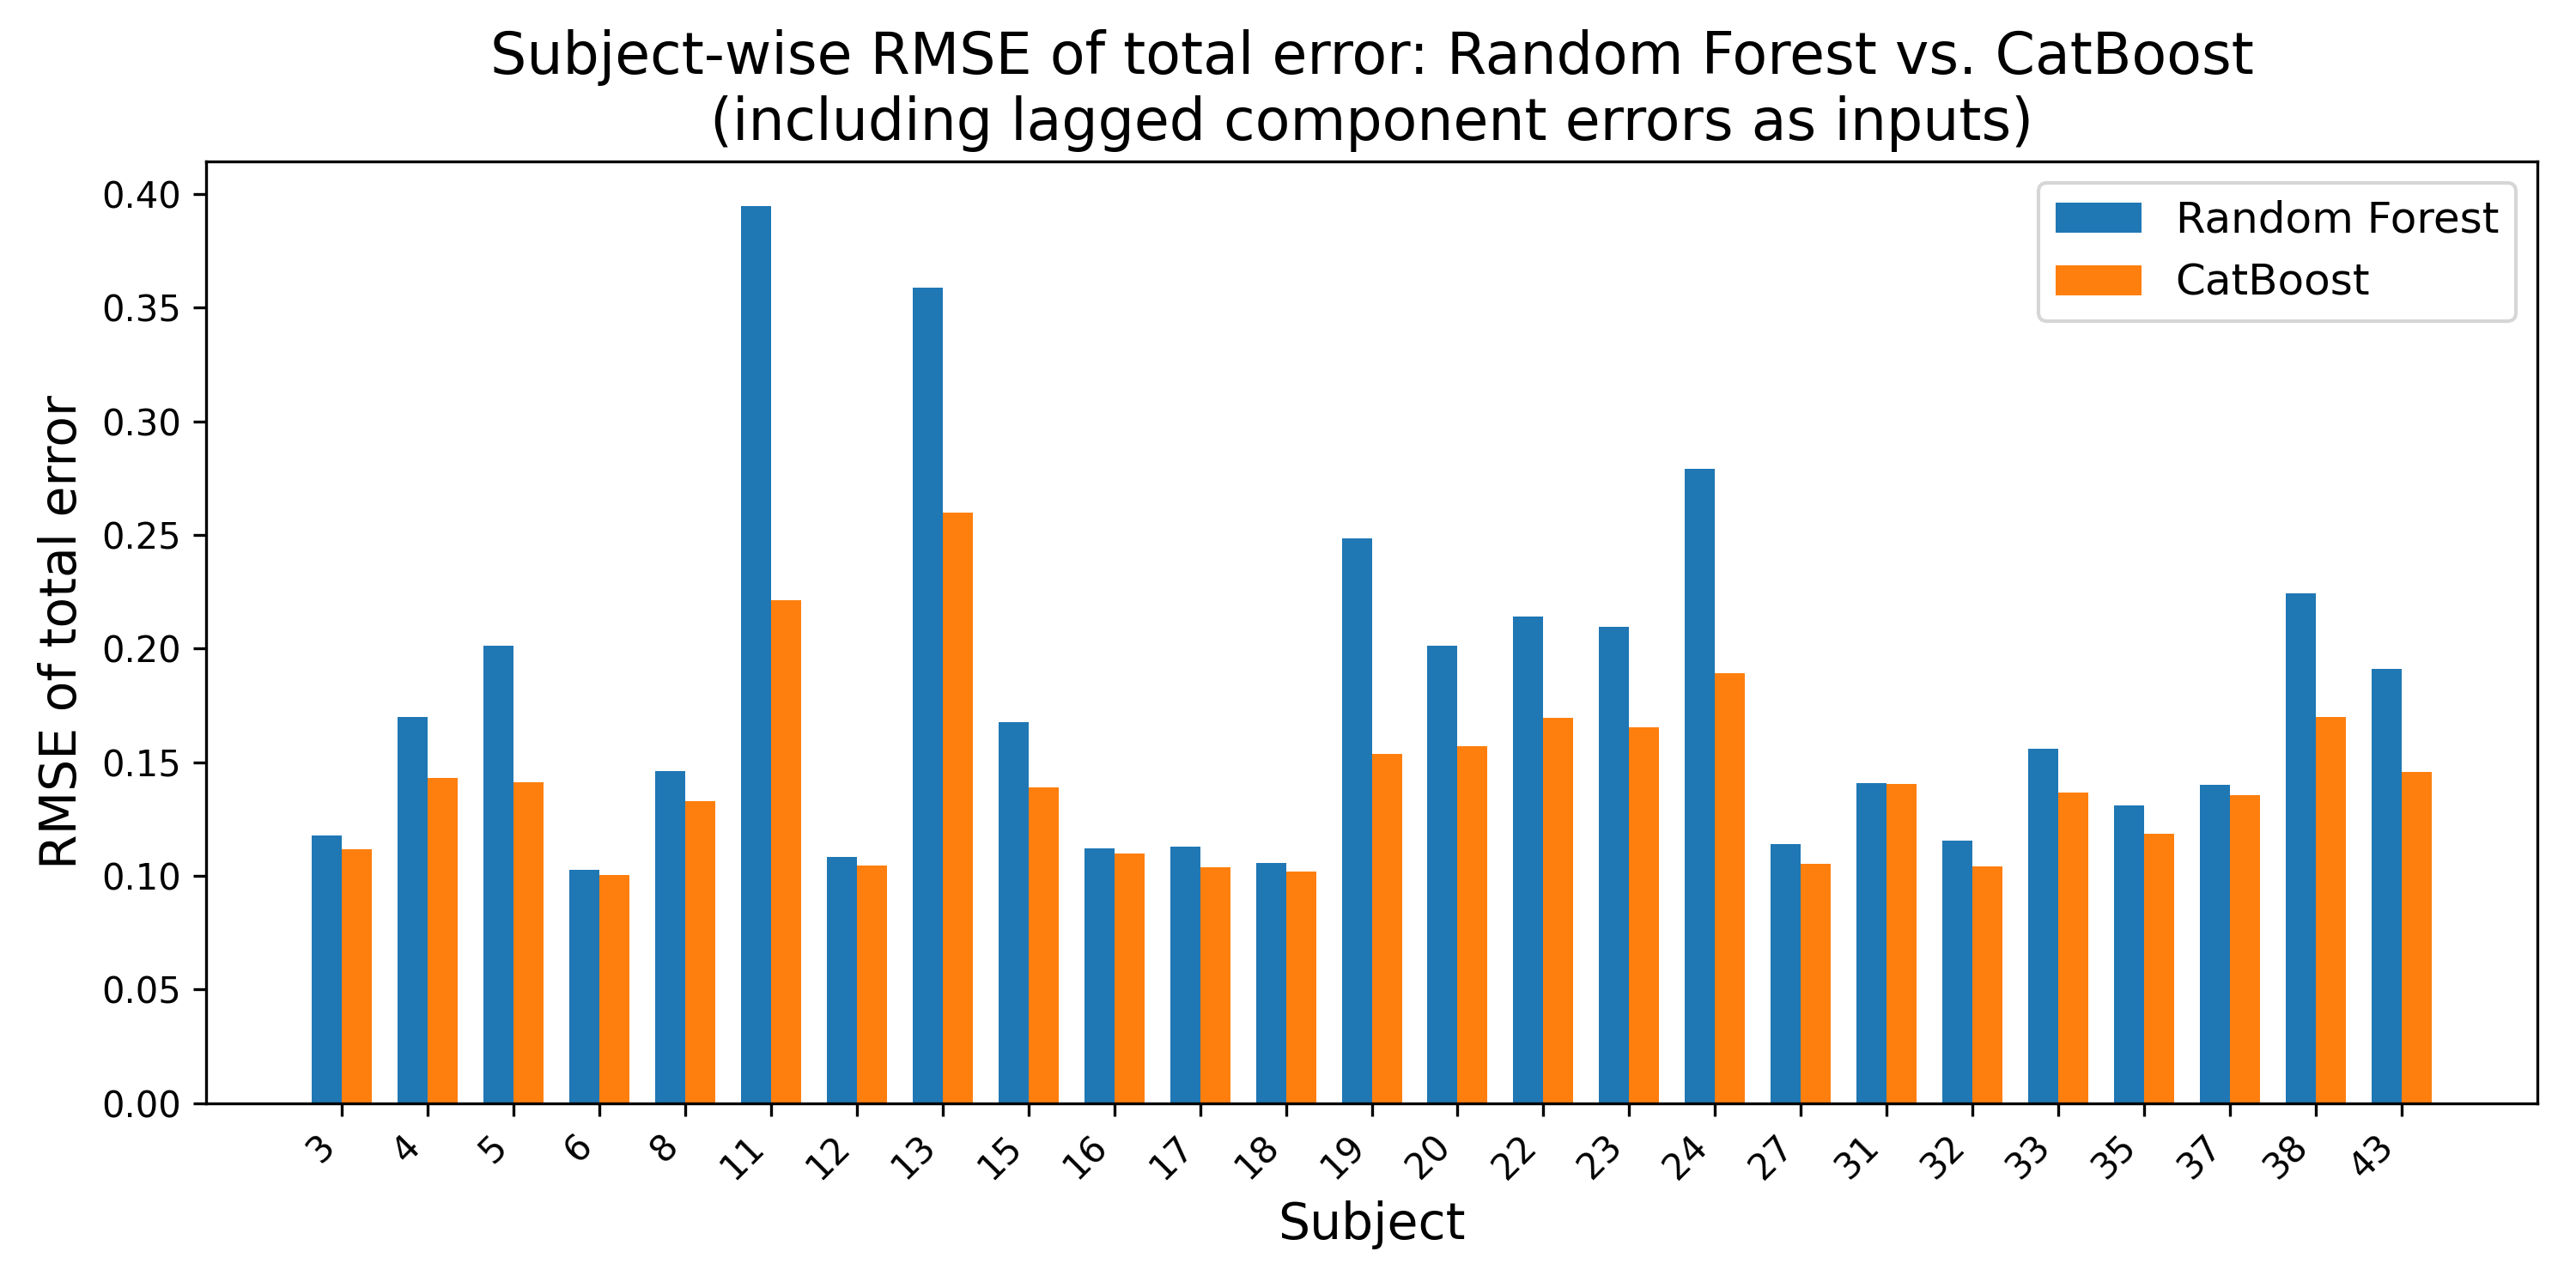
\includegraphics[width=\textwidth]{rmse_total_error_RF_vs_Cat_per_subject.png}
	\caption{Total-error RMSE (RF vs. CB)} 
	\label{fig:rmse-rf-vs-cb}
\end{figure}

\subsection{Generalization forward in time within a run}
Table~\ref{tab:model_perf_across_time} presents the generalization performance of the three models, averaged across output variables, with and without lagged error terms included as inputs. When the feature set contains only physiological and aircraft state variables, all models achieve modest predictive accuracy, with overall R$^2$ values between 0.16 and 0.19. Adding lagged component errors as inputs increases the overall R$^2$ to approximately 0.97 for Random Forest and about 0.98 for both XGBoost and CatBoost, while MAE and RMSE decrease by roughly a factor of 10. Among the three models, CatBoost with lagged features attains the lowest overall errors (MAE $\approx$ 0.07, RMSE $\approx$ 0.16).

\begin{table}[htbp]
	\caption{Model performance over the final 60 s of each run.}
	\label{tab:model_perf_across_time}
	\centering
	\small
	\begin{tabular}{p{3cm}llll}
		\toprule                                 	
		Input Condition 	&Model          	&  Mean MAE      &  Mean RMSE      & Mean R$^2$ \\ 
		\midrule
		\multirow{3}{*}{No lagged errors} &RF  & 0.72 & 1.17 & 0.16 \\
											&XGB & 0.77  	& 1.19  & 0.17 \\
											&CB   & 0.75  & 1.18 & 0.19 \\
		\midrule
		\multirow{3}{*}{With lagged errors} &RF   	& 0.10 	& 0.20 & 0.97 \\
											&XGB    & 0.09 	& 0.19 & 0.98 \\
											&CB  	& 0.07 	& 0.16 & 0.98 \\ 
		\bottomrule
	\end{tabular}
\end{table}

 Per-output predictive performance of the three models is shown in Table~\ref{tab:output_perf_no_lag}. When only physiological and aircraft state variables are used as inputs, all models exhibit modest accuracy, with R$^2$ values between approximately -0.2 and 0.4 and relatively large absolute errors. Nevertheless, the models capture some systematic variance, particularly for airspeed and total error, indicating that physiology and aircraft state alone provide limited but non-trivial information about upcoming deviations in tracking performance.

\begin{table}[htbp]
	\caption{Per-output predictive performance over the final 60 s of each run (no lagged component errors).}
	\label{tab:output_perf_no_lag}
	\centering
	\small
	\begin{tabular}{lllll}
		\toprule                                 	
		Model 	&Variable    & MAE      &  RMSE      &R$^2$ \\ 
		\midrule
		\multirow{4}{*}{RF} 		&Glide slope  	& 0.85 	 & 1.32  & 0.09	\\
									&Localizer			& 0.60	& 1.04	& -0.20 \\
									&Airspeed				& 0.48	& 0.82	& 0.34	\\
									&Total				&0.94	&1.52	&0.41	\\
									 
									   	    	
									
		\midrule
		\multirow{4}{*}{XGB} 		&Glide slope   &0.88  & 1.30 	& 0.11 \\
									&Localizer			&0.61 & 0.97 	& -0.05 \\
									&Airspeed				&0.51	& 0.84 	& 0.32  \\
									&Total				&1.08	 &1.67	 &0.29  \\
									     	  	
									
									
		\midrule 
		\multirow{4}{*}{CB} 		&Glide slope   & 0.87	 & 1.31	  	& 0.10	\\
									&Localizer     	& 0.60  & 0.96		& -0.03	\\
									&Airspeed				& 0.48 	& 0.82		& 0.35	\\
									&Total			&1.04	&1.62		&0.32	\\			
		\bottomrule
	\end{tabular}
\end{table}

Table~\ref{tab:output_perf_lag} reports per-output predictive performance when lagged component errors are included as inputs. In this configuration, predictive accuracy increases substantially: MAE and RMSE values decrease markedly, and R$^2$ values reach approximately 0.95 $-$ 0.99 for all outputs and models. CatBoost attains the lowest errors overall (e.g., total-error MAE $\approx$ 0.12, RMSE $\approx$ 0.21, R$^2$ $\approx$ 0.99), but Random Forest and XGBoost exhibit similar gains, underscoring the strong contribution of short-term error history to near-future performance prediction.

\begin{table}[htbp]
	\caption{Per-output predictive performance over the final 60 s of each run, including lagged component errors as inputs.}
	\label{tab:output_perf_lag}
	\centering
	\small
	\begin{tabular}{lllll}
		\toprule                                 	
		Model 	&Variable    & MAE      &  RMSE      &R$^2$ \\ 
		\midrule
		\multirow{4}{*}{RF} 	&Glide slope  	& 0.10 	 & 0.19  & 0.98	\\
								&Localizer			& 0.07	& 0.21	& 0.95 \\
								&Airspeed			& 0.09	& 0.15	& 0.98	\\
								&Total				&0.15	&0.27	&0.98	\\
		
		
		
		\midrule
		\multirow{4}{*}{XGB} 		&Glide slope   &0.09   & 0.18 	& 0.98 \\
									&Localizer		&0.07 & 0.20 	& 0.96 \\
									&Airspeed		&0.07	& 0.12 	& 0.99  \\
									&Total			&0.15	 &0.26	 &0.98  \\
		
		
		
		\midrule 
		\multirow{4}{*}{CB} 		&Glide slope   & 0.06	 & 0.15	  	& 0.99	\\
									&Localizer     	& 0.05  & 0.18		& 0.96	\\
									&Airspeed		& 0.06 	& 0.11		& 0.99	\\
									&Total			&0.12	&0.21		&0.99	\\			
		\bottomrule
	\end{tabular}
\end{table}

Comparing Tables \ref{tab:sub-overall} and \ref{tab:model_perf_across_time} shows that generalization to unseen pilots is somewhat more difficult than generalization to the final 60 s within a run. In both feature-set configurations, all models achieve higher R$^2$ when generalizing forward in time than when generalizing across individuals. This pattern suggests that individual pilots exhibit relatively consistent short-term dynamics that can be exploited to anticipate upcoming deviations, whereas cross-subject variability remains more challenging for the models to capture.

\subsection{Error Correlations and Feature Importance}
Table~\ref{tab:corr-comp-total} reports Pearson correlations between true component errors and true total error. The true data show only weak associations between individual component errors and total error, indicating that overall error combines several largely distinct parts rather than being dominated by a single component. Correlations between predicted individual errors and true total error are presented in Table~\ref{tab:corr_pred_total_no_lag} and Table~\ref{tab:corr_pred_total_lag} in Appendix A. In both generalization schemes without lagged component errors as inputs, these correlations are small and do not reproduce the correlation pattern observed in the true data, suggesting that the models fail to capture the true multicomponent structure of overall error. Figure~\ref{fig:corr-no-lag} illustrates this discrepancy.

\begin{table}[htbp]
	\caption{Pearson correlations between true component errors and true total error}
	\label{tab:corr-comp-total}
	\centering
	\small
	\begin{tabular}{lcc}
		\toprule
		Component Error	& Pearson $r$ (across subjects)	& Pearson $r$ (across time)  \\ 
		\midrule
		Glide Slope  	& 0.09 & 0.11\\
		Localizer        & -0.20 & -0.11\\
		Airspeed  	& 0.22 & 0.20\\
		\bottomrule
	\end{tabular}
\end{table}

In contrast, all three models match the observed correlation pattern more closely when lagged component errors are included as inputs. For both generalization strategies, the correlations between predicted component errors and true total error closely resemble the corresponding correlations in the true data. The correlation between predicted and true total error reaches 0.99 for all models. These results suggest that the models reproduce the observed relationships between the individual error components and overall approach performance. Figure~\ref{fig:corr-lag} illustrates these relationships for the CatBoost model, showing that the regression lines for the predicted component errors closely track those of the true errors across the range of total error.


\begin{figure}[htbp]
	\centering
	
\includegraphics[width=\textwidth]{corr_vs_true_total_error.png}
	\caption{Correlations between predicted component errors and the true total error (CatBoost generalization across time without lagged error inputs).}
	\label{fig:corr-no-lag}
\end{figure}

Feature importance analyses for the models without lagged error inputs (Table~\ref{tab:feat_imp_subject_no_lag} and Table~\ref{tab:feat_imp_time_no_lag} in Appendix A) showed that physiological variables related to heart rate and respiration rate, together with several aircraft state variables, were the most influential predictors of the performance variables. For example, in both the Random Forest and XGBoost models, mean elevation trim and mean aileron trim received the highest importance scores, followed by heart-rate range and breathing-related features.

\begin{figure}[htbp]
	\centering
	
\includegraphics[width=\textwidth]{corr_vs_true_total_error_lag.png}
	\caption{Correlations between predicted component errors and the true total error (CatBoost generalization across time with lagged error inputs).}
	\label{fig:corr-lag}
\end{figure}

After adding lagged error variables as inputs, the importance pattern changed substantially (Table \ref{tab:feat-imp-sub-lag} and Table \ref{tab:feat-imp-temp-lag} in Appendix A). In all three models, lagged component error variables became the primary predictors: component errors at time t-1 received the highest importance, whereas component errors at time t-2 and most physiological and aircraft features had much smaller importance scores. This pattern suggests that short-term performance history is the strongest predictor of current errors, with aircraft and physiological variables providing additional but comparatively modest contributions.

SHAP value analyses were used to examine these patterns in more detail. Consistent with the feature-importance results for models without lagged error inputs, the SHAP summary plot for total error showed that aircraft state variables and physiology-related variables dominated the predictions (Figure \ref{fig:shap-catboost-temp} in Appendix A). In particular, higher elevation trim and aileron trim values, together with larger heart-rate range and respiration-related features, were associated with increased predicted total error.

When lagged component errors were added as inputs, SHAP values showed that component errors at time t-1 were by far the largest contributors to predicted total error, whereas component errors at time t-2 and most physiological and aircraft variables had much smaller SHAP magnitudes (Figure \ref{fig:shap-catboost-temp-lag} in Appendix A). This pattern aligns with the feature-importance analyses and suggests that short-term performance history over the previous 1 to 2 seconds is the primary driver of the model’s predictions.


\section{Discussion}
This section presents an evaluation of the results obtained from the three tree‑based regression models for forecasting performance errors, and discusses the limitations of the study as well as directions for future research.

\subsection{Main Findings}
This thesis examined how accurately pilots’ tracking performance during virtual reality landing approaches can be predicted in near real time from multimodal physiological and simulator-derived features using tree-based regression models. When only physiological and aircraft state variables were included as inputs, all three models achieved at best modest predictive accuracy: in the across-subject generalization setting, overall R$^2$ values were negative, indicating performance below a mean-baseline predictor, and in the across-time generalization setting, overall R$^2$ values reached only about 0.16–0.19. In contrast, adding lagged component errors at times t-1 and t-2 as input features led to a substantial increase in explained variance in both generalization settings, with overall R$^2$ values of approximately 0.95$-$0.99 and MAE and RMSE reduced to around one-tenth of their values in the corresponding conditions. These results indicate that, for this task, when the system is able to continuously record recent performance history, models can track performance with high precision. Models relying solely on physiology and aircraft state still provide limited but non-negligible information about moment-to-moment deviations in performance, particularly after patterns of an individual pilot have been observed.

Differences among the three tree-based models were small compared with the gains from including lagged error features. CatBoost consistently attained the lowest overall MAE and RMSE and the highest R$^2$ values, but Random Forest and XGBoost exhibited very similar performance when given the same feature sets, suggesting that access to short-term error history is more critical for prediction quality than the specific model architecture. Analyses of error correlations further showed that, in the true data, individual component errors were only weakly associated with total error, indicating that overall performance reflects a combination of distinct error sources rather than being dominated by a single component. When lagged errors were included, all three models closely reproduced both the observed error correlations and the high correlation between predicted and true total error, suggesting that they captured the multicomponent structure of approach performance rather than merely fitting individual outputs in isolation.

Feature-importance analyses and SHAP value inspections supported this interpretation. Without lagged error inputs, aircraft state variables such as mean elevation and aileron trim, together with heart-rate range and respiration-related features, were the most influential predictors. After adding lagged component errors, the importance pattern shifted markedly: component errors at the previous time steps became the dominant predictors, whereas most physiological and aircraft variables contributed relatively little additional information.

Comparing the two generalization schemes revealed that predicting forward in time for the same individual is easier than generalizing to unseen subjects. Across all feature configurations and models, R$^2$ values were consistently higher in the within-run, across-time setting than in the across-subject setting, and variability in error metrics across individuals remained substantial even when lagged errors were included. This pattern suggests that individual pilots exhibit relatively stable short‑term dynamics that can be exploited to anticipate upcoming deviations within a run, whereas cross‑subject variability in physiology and aircraft control strategies poses a greater challenge for the models and limits their ability to generalize to new pilots.

From an applied perspective, these findings suggest that adaptive training systems are most effective when they can continuously track and exploit each trainee’s recent performance history, whereas models that must generalize to new pilots using only physiology and aircraft state provide more limited predictive reliability.

\subsection{Relation to Prior Work}
Prior research in simulated and VR flight has shown that ECG-derived heart rate and respiration measures covary with mental workload, stress, and overall performance\cite{koerner-2025,bruna-2018,grassmann-2016}, and can be used to differentiate task conditions or performance levels \cite{caballero-2023, moore-2023}. This work is broadly consistent with the present findings in that heart-rate and respiration-based features received non-zero importance in models that relied only on physiology and aircraft state. At the same time, the current results qualify earlier conclusions by demonstrating that, once very short-term performance history is available, physiological variables contribute relatively little additional predictive power to near-future error prediction. In other words, physiology appears informative when recent performance is unknown, but its unique value diminishes when recent tracking errors can be measured directly.

The present study also extends earlier analyses on this specific dataset that focused on classifying discrete difficulty levels or predicting offline summary measures of landing performance. Previous models have shown that subsets of physiological and eye-tracking signals can distinguish flight-difficulty conditions \cite{caballero-2023, moore-2023}, and that tree-based models trained on aggregated features can predict overall landing-error metrics \cite{barry-2025}. The current work goes beyond these approaches in several respects: it treats landing performance as a continuous multivariate time series rather than as a single summary score, uses multi-output regression to predict the full trajectory of component and total errors at a one-second horizon, and evaluates performance under both generalization to new subjects and generalization forward in time within the same run. In this study, simple one- and two-second lagged component error terms enable very high explained variance. This suggests that, for short-horizon prediction, recent performance history is a more critical predictor than was emphasized in prior classification- and summary-level regression studies on the same data.


\subsection{Methodological Considerations and Limitations}
The generalizability of these findings is constrained by several methodological choices. First, all analyses were conducted on a relatively small sample of participants performing a single VR ILS landing task, which may limit the extent to which the models transfer to other training scenarios or populations. Second, the models focused on very short time‑window prediction using one‑ and two‑step lagged error and feature values; longer‑horizon forecasting may reveal a stronger role for physiological dynamics, as McGuire \emph{et al.} \cite{mcguire-2026} showed that physiological signals can estimate errors up to 10 seconds before they occur in real‑world flight operations. Third, the feature engineering pipeline used manually designed summary statistics and lagged features instead of end‑to‑end temporal models that learn directly from raw time‑series data. 

A further methodological consideration concerns how realistic the most accurate model configuration is for real-time flight training. Although models that include lagged component errors achieve near-perfect predictive accuracy, this setup relies on continuous access to recent performance, which may not always be available, reliable, or desirable in operational training environments.

\subsection{Implications and Future Directions}
The present findings inform how data-driven support tools in flight training might balance different information sources. The near-perfect accuracy achieved when using lagged component errors indicates that recent performance history is a powerful cue for short-horizon prediction, and that even comparatively simple tree-based models can exploit it effectively. However, this should be interpreted primarily as a proof of principle for what is achievable under ideal conditions, because it presupposes continuous, high-quality access to recent performance data, which may not be accessible  in all training devices or operational settings. In contrast, when relying solely on physiological and aircraft state variables, the models achieve modest but non-trivial predictive accuracy for generalization forward in time within a run, indicating that these signals do contain information about upcoming deviations in tracking performance. This pattern suggests that physiology-based predictors may support forward‑in‑time performance monitoring for trainee pilots when recent error history is unavailable, delayed, or noisy, even though they do not reach the same level of accuracy as models that exploit short-term error history.

From an applied perspective, these results point towards different roles for performance-history and physiology-based predictors in adaptive training systems. In high-fidelity VR simulators where detailed performance traces are readily available, models that integrate lagged errors with a small set of aircraft and physiological variables could underpin intelligent instructor systems that provide short-term forecasts of pilot performance, and support scalable, objective assessment. In settings where performance metrics are less complete or delayed, such as certain operational environments or lower-fidelity training devices, physiology-driven models may instead provide a complementary channel for anticipating upcoming performance degradation. Designing adaptive systems that can flexibly combine these information sources depending on what is available in real time is a promising direction for future work.

Future research could extend this work in multiple directions. First, evaluating models for longer‑horizon performance prediction would provide insight into how far ahead performance errors can be forecast, and whether physiological dynamics contribute more strongly when predicting several seconds into the future. Second, applying the modeling framework to other VR flight tasks or datasets, including scenarios with different levels of difficulty, environmental conditions, or trainee expertise, would help assess robustness and external validity. Finally, integration of such models into live VR training sessions could help study their impact on instructor workload, trainee learning curves, and relevant safety behavior while providing empirical evidence on whether physiology‑informed performance prediction meaningfully improves training efficiency and operational safety outcomes.


\section{Conclusion}
This thesis investigated how accurately pilots' performance during a virtual reality ILS landing task can be predicted in near real time using tree-based regression models trained on multimodal physiological and simulator-derived features. The analysis addressed two sub-questions: to what extent short-term performance history improves predictive accuracy, and which inputs contribute most to prediction performance in the trained models.

The results showed that models can predict performance errors with high accuracy in both generalization across subjects and generalization forward in time within the same trial when lagged component errors are available as inputs, and these lagged errors emerge as the most influential predictors. When the feature set contains only physiological and aircraft state variables, overall explained variance remains modest, though these variables still achieve limited but non-trivial predictive power, further confirming that physiological signals relate to task demand and performance. Taken together, these findings indicate that short-term performance history substantially increases predictive accuracy when a continuous record of recent errors is available online, while physiology- and aircraft-related information is still relevant in situations where performance data are unavailable, delayed, or noisy.

Overall, the findings suggest that tree-based regression models can serve as one component in adaptive and scalable training systems in VR-based settings. However, the design of such systems in aviation should carefully consider the training environment and the availability and reliability of different signal types. Future research should therefore examine physiological dynamics in both simulated and operational environments, apply the modeling framework to diverse tasks and trainee populations, and evaluate closed-loop implementations in which performance- and physiology-informed predictions are integrated into live VR or operational training, in order to assess their impact on learning, workload, and safety-relevant behavior.


\bibliography{references}

\clearpage
\appendix
\markboth{APPENDIX A}{APPENDIX A}
\section*{Appendix A} 
\label{app:a}

\begin{table}[htbp]
	\caption{Overview of multimodal physiological data}
	\label{tab:multimodal}
	\centering
	\small
	\begin{tabular}{lllp{2cm}}
		\toprule                                 	
		Variable Name         &Unit           &Sampling Rate        		&  Description     \\ 
		\midrule
		EMG Wrist Flexor 	&mV  				& 128 Hz         	& EMG of wrist flexor muscles\\
		\midrule
		EMG Wrist Extensor 	&mV				& 512 HZ         & EMG of wrist extensor muscles  \\
		\midrule  			
		PPG Finger 	&mV				&128 Hz     & Optical signal at tip of the middle finger \\
		\midrule
		EDA Hand L &KOhms 				& 1024 Hz          		& EDA measured on the left hand \\
		\midrule
		ECG Projection LL-RA &mV     &128 Hz           		& ECG Signal: LL-RA projection \\
		\midrule
		ECG Projection LA-RA &mV    &128 Hz          		& ECG Signal: LA-RA projection \\
		\midrule
		ECG Projection VX-RL &mV    &128 Hz           		& ECG Signal: VX-RL projection \\
		\midrule
		Respiration Trace &mV    	&128 Hz        		& Respiration Trace \\
		\midrule
		Accelerometry Forearm x/y/z &\text{m/s\textsuperscript{2}}    &128 Hz  & Accelerometry of the right forearm\\
		\midrule
		Accelerometry Torso x/y/z &\text{m/s\textsuperscript{2}}   &128 Hz  & Accelerometry of the torso\\
		\midrule
		Gaze Origin L/R x/y/z &mm		&250 Hz 		& Origin point of the gaze ray from each eye \\
		\midrule
		Gaze Direction L/R x/y/z &mm	&250 Hz		& The normalized gaze direction of each eye \\
		\midrule
		Eye Openness L/R &$-$			&250 Hz  		& A value representing how open each eye is\\
		\midrule
		Pupil Position L/R x/y/z &$-$	&250 Hz  	& Position of each pupil in sensor area\\
		\midrule
		Pupil Diameter L/R  &mm			&250 Hz 		& Diameter of each pupil\\
		\bottomrule	
	\end{tabular}
\end{table}

\begin{table}[htbp]
	\caption{Pearson correlations between predicted individual errors and true total error (without lagged error inputs)}
	\label{tab:corr_pred_total_no_lag}
	\centering
	\small
	\begin{tabular}{llcc}
		\toprule
		                     
		Model     & Variable  & Pearson $r$ (across subjects)	& Pearson $r$ (across time)   \\ 
		\midrule
		\multirow{4}{*}{RF}  	&Glide slope  	& -0.07 & 0.09 	\\
								&Localizer		& 0.04	& -0.01	 \\
								&Airspeed		& 0.11	& 0.17	\\
								&Total			& 0.28	&0.69	\\	
		\midrule
		\multirow{4}{*}{XGB}    & Glide slope 	&-0.07   	& 0.16\\
								& Localizer 	& 0.04 		& -0.14\\
								& Airspeed 		& 0.04  	& 0.16\\
								& Total 		& 0.24 		& 0.61\\
		\midrule
		\multirow{4}{*}{CB}  	& Glide slope 	&-0.10   & 0.17\\
								& Localizer 	& -0.01 & -0.07\\
								& Airspeed 		& 0.05  & 0.18\\
								& Total 		& 0.22 & 0.64\\
		\bottomrule
	\end{tabular}
\end{table}

\begin{table}[htbp]
	\caption{Pearson correlations between predicted individual errors and true total error (with lagged error inputs)}
	\label{tab:corr_pred_total_lag}
	\centering
	\small
	\begin{tabular}{llcc}
		\toprule
		
		Model     & Variable  & Pearson $r$ (across subjects)	& Pearson $r$ (across time)   \\ 
		\midrule
		\multirow{4}{*}{RF}  	&Glide slope  	& 0.09 & 0.10 	\\
								&Localizer		& -0.20	& -0.12	 \\
								&Airspeed		& 0.23	& 0.21	\\
								&Total			& 0.99	&0.99	\\	
		\midrule
		\multirow{4}{*}{XGB}    & Glide slope 	&0.09   	& 0.10\\
								& Localizer 	&-0.20 		& -0.142\\
								& Airspeed 		& 0.22  	& 0.21\\
								& Total 		& 0.99 		& 0.99\\
		\midrule
		\multirow{4}{*}{CB}  	& Glide slope 	&0.09   & 0.10\\
								& Localizer 	& -0.20 & -0.11\\
								& Airspeed 		& 0.22  & 0.21\\
								& Total 		& 0.99 & 0.99\\
		\bottomrule
	\end{tabular}
\end{table}

\begin{table}[htbp]
	\centering
	\caption{Feature importance for predicting performance error without lagged error inputs (across-subject generalization).}
	\label{tab:feat_imp_subject_no_lag}
	\small
	\begin{tabular}{llc}
		Model & Feature  & Importance Value\\
		\midrule
		\multirow{12}{*}{Random Forest} &Mean Elevation & 0.247\\
										&HR Range       & 0.094\\
										&Mean Aileron         & 0.127\\
										&Level     	& 0.053 \\
										&Mean HR             & 0.066\\
										&Mean BR             & 0.075\\
										&SD BR              & 0.054\\
										&Max HR              & 0.059 \\
										&Min HR              & 0.078\\
										&SD HR             & 0.035\\
										&Mean RESP Amp       & 0.071\\
										&SD RESP Amp        & 0.042 \\								
		\midrule
		\multirow{12}{*}{XGBoost}		&Mean Elevation & 0.222\\
										&HR Range       & 0.062\\
										&Mean Aileron         & 0.138\\
										&Level      & 0.134 \\
										&Mean HR             & 0.036\\
										&Mean BR             & 0.050\\
										&SD BR              & 0.046\\
										&Max HR             & 0.117 \\
										&Min HR              & 0.052 \\
										&SD HR             & 0.066\\
										&Mean RESP Amp       & 0.052\\
										&SD RESP Amp		& 0.026 \\
		\midrule											 
		\multirow{12}{*}{CatBoost}		&Mean Elevation & 33.716 \\
										&HR Range       & 18.277 \\
										&Mean Aileron         & 12.434 \\
										&Level      &  10.610 \\
										&Mean HR             &  4.601\\
										&Mean BR             &  4.426 \\
										&SD BR              &  3.813 \\
										&Max HR             &  5.350 \\
										&Min HR              &  1.206 \\
										&SD HR             &  0.418 \\
										&Mean RESP Amp       &  5.150 \\
										&SD RESP Amp		&  0.000 \\				
		\bottomrule
	\end{tabular}
\end{table}

\begin{table}[htbp]
	\centering
	\caption{Feature importance for predicting performance error without lagged error inputs (across-time generalization).}
	\label{tab:feat_imp_time_no_lag}
	\small
	\begin{tabular}{llc}
		\toprule
		Model & Feature  & Importance Value\\
		\midrule
		\multirow{12}{*}{Random Forest} &Mean Elevation & 0.248\\
										&HR Range       & 0.089\\
										&Mean Aileron         & 0.131\\
										&Level     & 0.056 \\
										&Mean HR             & 0.062\\
										&Mean BR             & 0.075\\
										&SD BR              & 0.055\\
										&Max HR              & 0.061\\
										&Min HR              & 0.072\\
										&SD HR             & 0.036\\
										&Mean RESP Amp       & 0.074\\
										&SD RESP Amp        & 0.041\\								
		\midrule
		\multirow{12}{*}{XGBoost}		&Mean Elevation & 0.154\\
										&HR Range       & 0.066\\
										&Mean Aileron         & 0.112\\
										&Level      & 0.136 \\
										&Mean HR             & 0.059\\
										&Mean BR             & 0.050\\
										&SD BR              & 0.048\\
										&Max HR             & 0.010 \\
										&Min HR              & 0.051 \\
										&SD HR             & 0.146\\
										&Mean RESP Amp       & 0.046\\
										&SD RESP Amp		& 0.033 \\
		\midrule											 
		\multirow{12}{*}{CatBoost}		&Mean Elevation & 30.065 \\
										&HR Range       & 11.620 \\
										&Mean Aileron         & 14.929 \\
										&Level      &  9.593 \\
										&Mean HR             &  7.272 \\
										&Mean BR             &  6.898 \\
										&SD BR              &  4.088 \\
										&Max HR             &  5.102 \\
										&Min HR              &  3.417 \\
										&SD HR             &  0.614 \\
										&Mean RESP Amp       &  6.259 \\
										&SD RESP Amp		&  0.143 \\				
		\bottomrule
	\end{tabular}
\end{table}

\begin{table}[htbp]
	\caption{Feature importance for predicting performance error with lagged error inputs (across-subject generalization).}
	\label{tab:feat-imp-sub-lag}
	\centering
	\small
	\begin{tabular}{llc}
		\toprule
		Model & Feature & Importance Value \\
		\midrule
		\multirow{7}{*}{Random Forest} 	& Glide slope error (t-1) &0.513\\
										& Airspeed error (t-1)    & 0.247\\
										& Localizer error (t-1) 	&0.223\\
										&Localizer error (t-2)		&0.011\\
										&Glide slope error (t-2)	&0.002\\
										&Airspeed error (t-2)		&0.001\\
										&Mean RESP Amp 				&0.001\\
		\midrule
		\multirow{7}{*}{XGBoost} 		&Airspeed error (t-1)		& 0.276\\
										&Glide slope error (t-2)	&0.257\\
										&Localizer error (t-1)		&0.206\\
										&Glide slope error (t-1)	&0.124\\
										&Localizer error (t-2)		&0.070\\
										&Mean elevation 			&0.025\\
										&Mean aileron				&0.011\\
		\midrule
		\multirow{7}{*}{CatBoost}		&Glide slope error (t-1)	&39.610\\
										&Airspeed error (t-1)		&26.973\\
										&Localizer error (t-1)		&17.852\\
										&Glide slope error (t-2)	&8.069\\
										&Localizer error (t-2)		&6.767\\
										&Airspeed error (t-2)		&0.712\\
										&Mean elevation 			&0.006\\
		\bottomrule
	\end{tabular}
\end{table}

\begin{table}[htbp]
	\caption{Feature importance for predicting performance error with lagged error inputs (across-time generalization).}
	\label{tab:feat-imp-temp-lag}
	\centering
	\small
	\begin{tabular}{llc}
		\toprule
		Model & Feature & Importance Value \\
		\midrule
		\multirow{7}{*}{Random Forest} &Glide slope error (t-1) &0.388\\
										&Airspeed error (t-1)  &0.279\\
										&Localizer error (t-1) &0.229\\
										&Glide slope error (t-2) &0.081\\
										&Localizer error (t-2)	&0.016\\
										&Airspeed error (t-2)  &0.001\\
										&Mean RESP amp			&0.001\\
		\midrule
		\multirow{7}{*}{XGBoost} 		&Airspeed error (t-1)		& 0.280\\
										&Glide slope error (t-2)	&0.247\\
										&Localizer error (t-1)		&0.196\\
										&Glide slope error (t-1)	&0.126\\
										&Localizer error (t-2)		&0.073\\
										&Mean elevation 			&0.025\\
										&Max HR						&0.011\\
		\midrule
		\multirow{7}{*}{CatBoost}		&Airspeed error (t-1)		&26.973\\
										&Glide slope error (t-1)	&26.645\\
										&Localizer error (t-1)		&16.689\\
										&Glide slope error (t-2)	&15.932\\
										&Localizer error (t-2)		&10.958\\
										&Airspeed error (t-2)		&2.340\\
										&Mean elevation 			&0.011\\
		\bottomrule
	\end{tabular}
\end{table}

\begin{figure}[htbp]
	\centering
	\begin{subfigure}{0.48\textwidth}
		\centering
		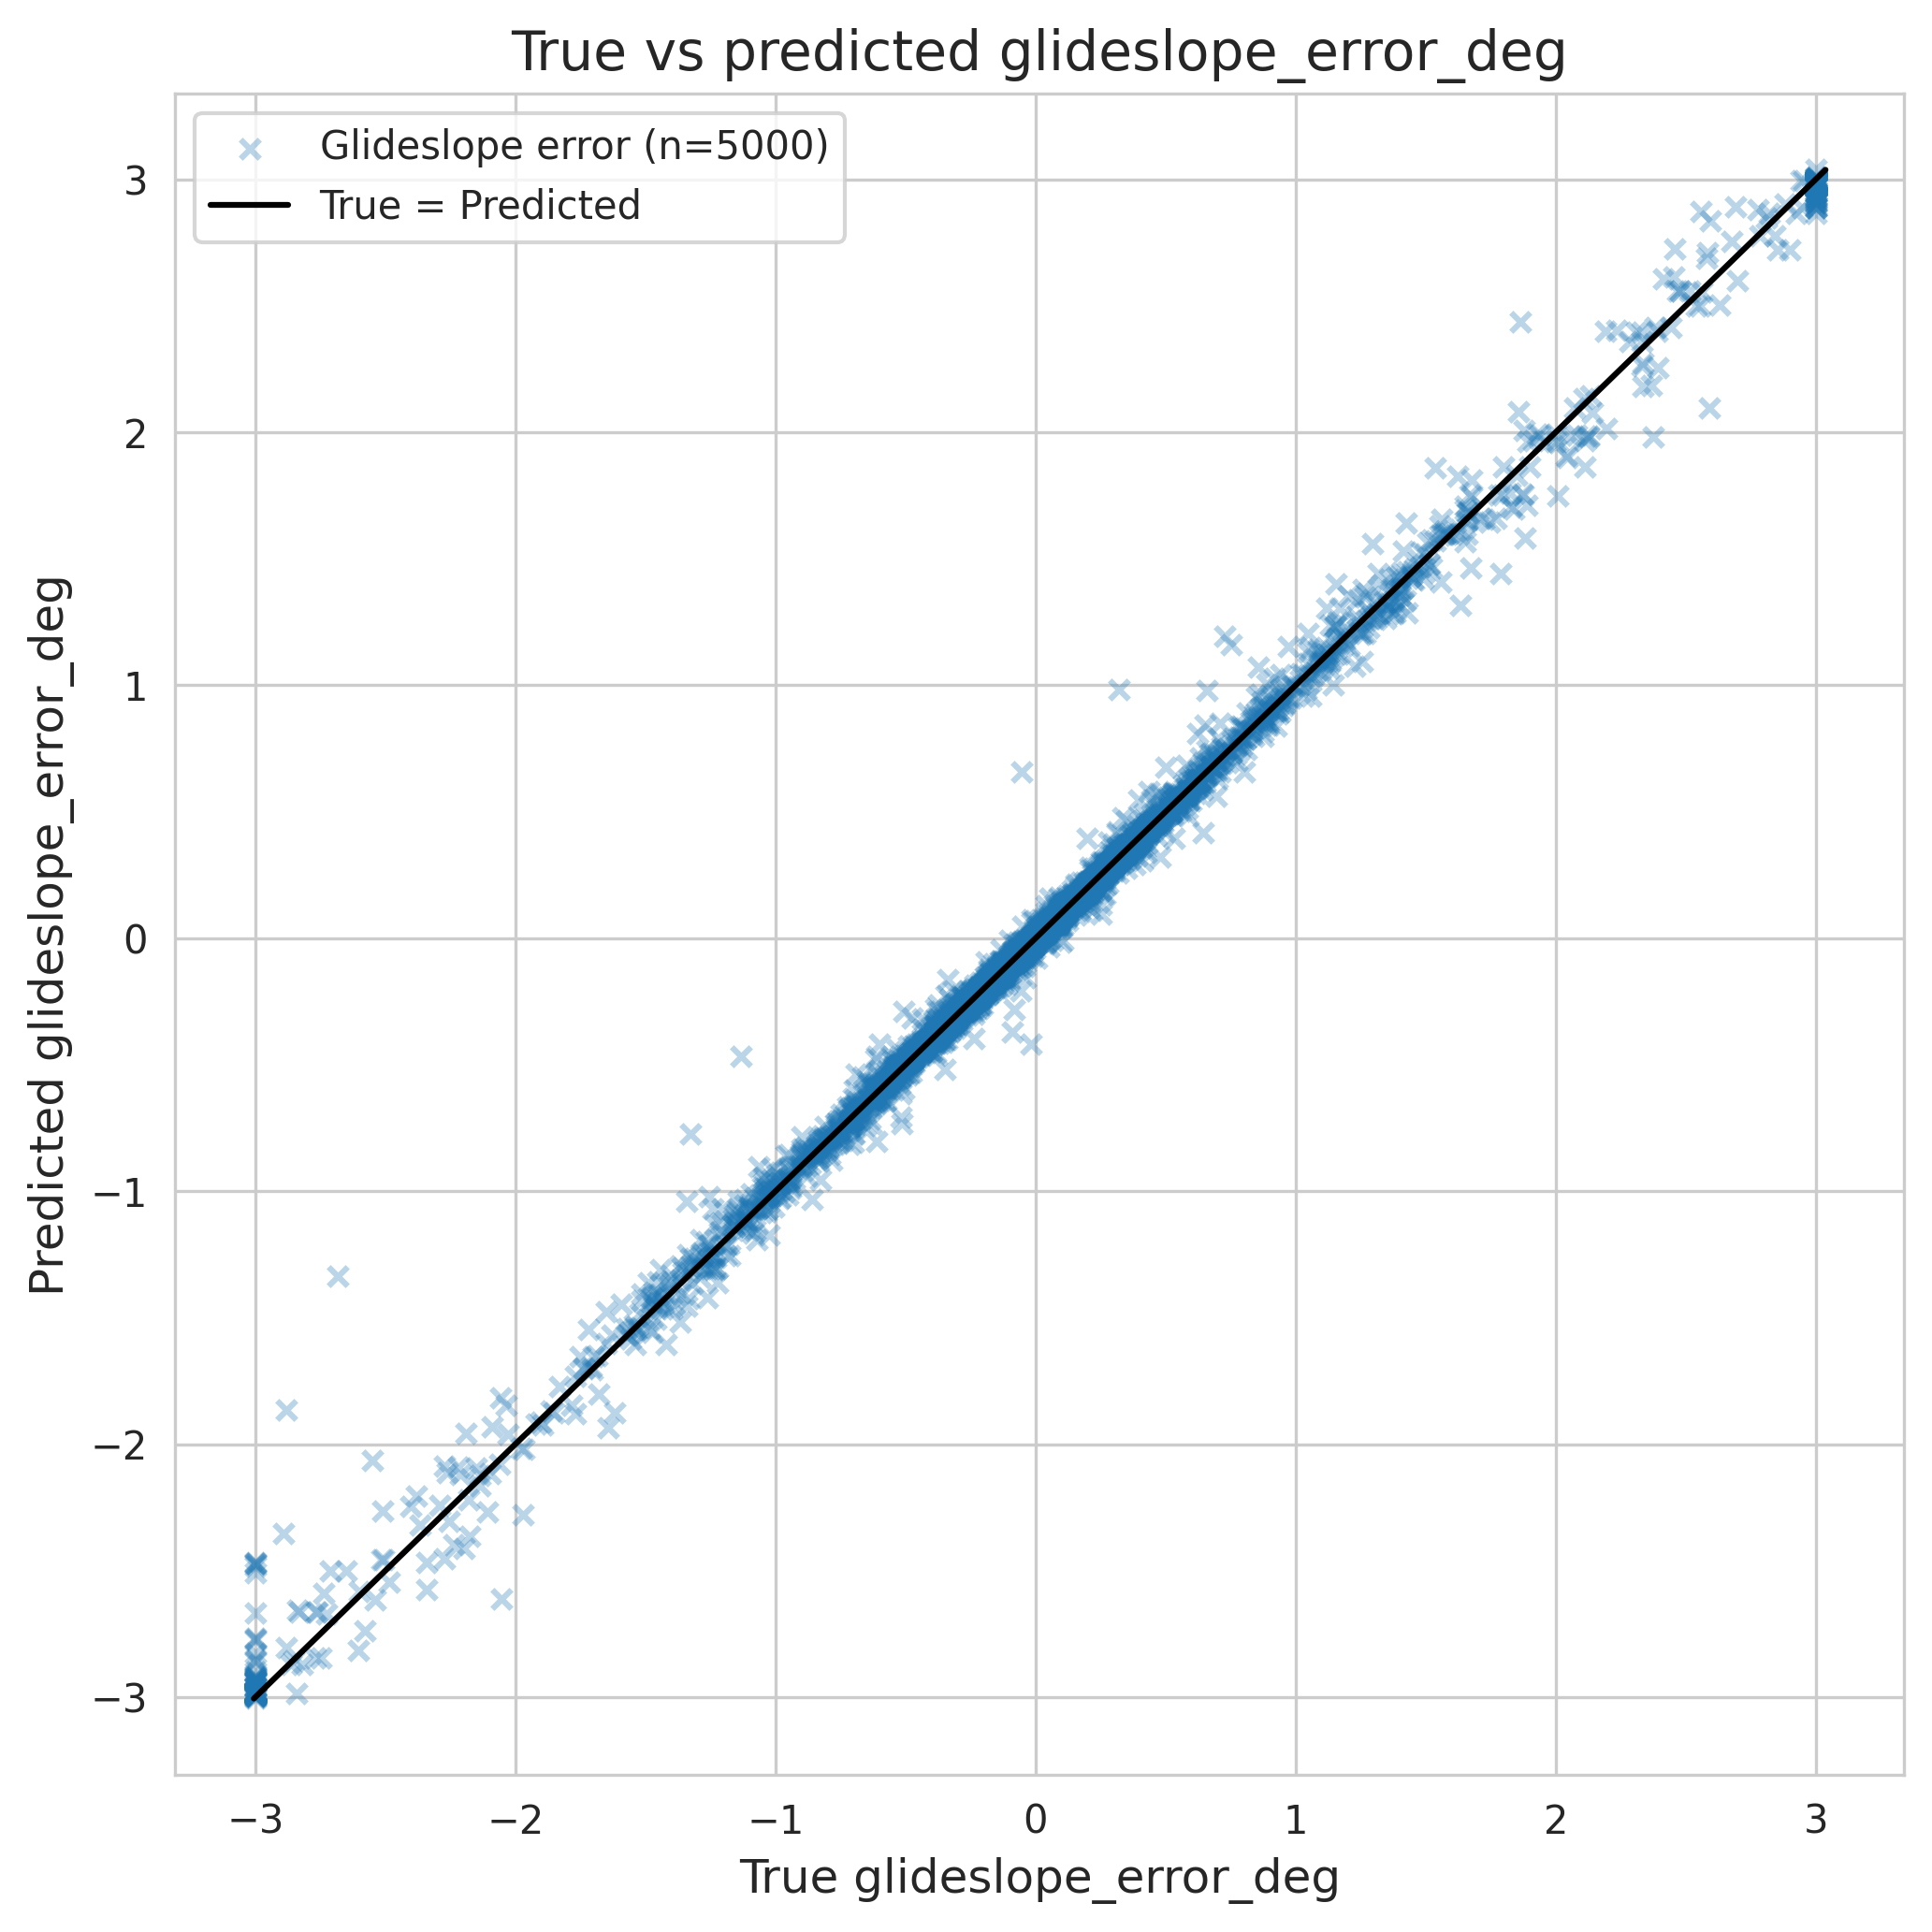
\includegraphics[width=\linewidth]{scatter_true_vs_pred_glideslope_error_deg_lag.png}
		\caption{Glide slope}
		\label{fig:sub-glide}
	\end{subfigure}
	\begin{subfigure}{0.48\textwidth}
		\centering
		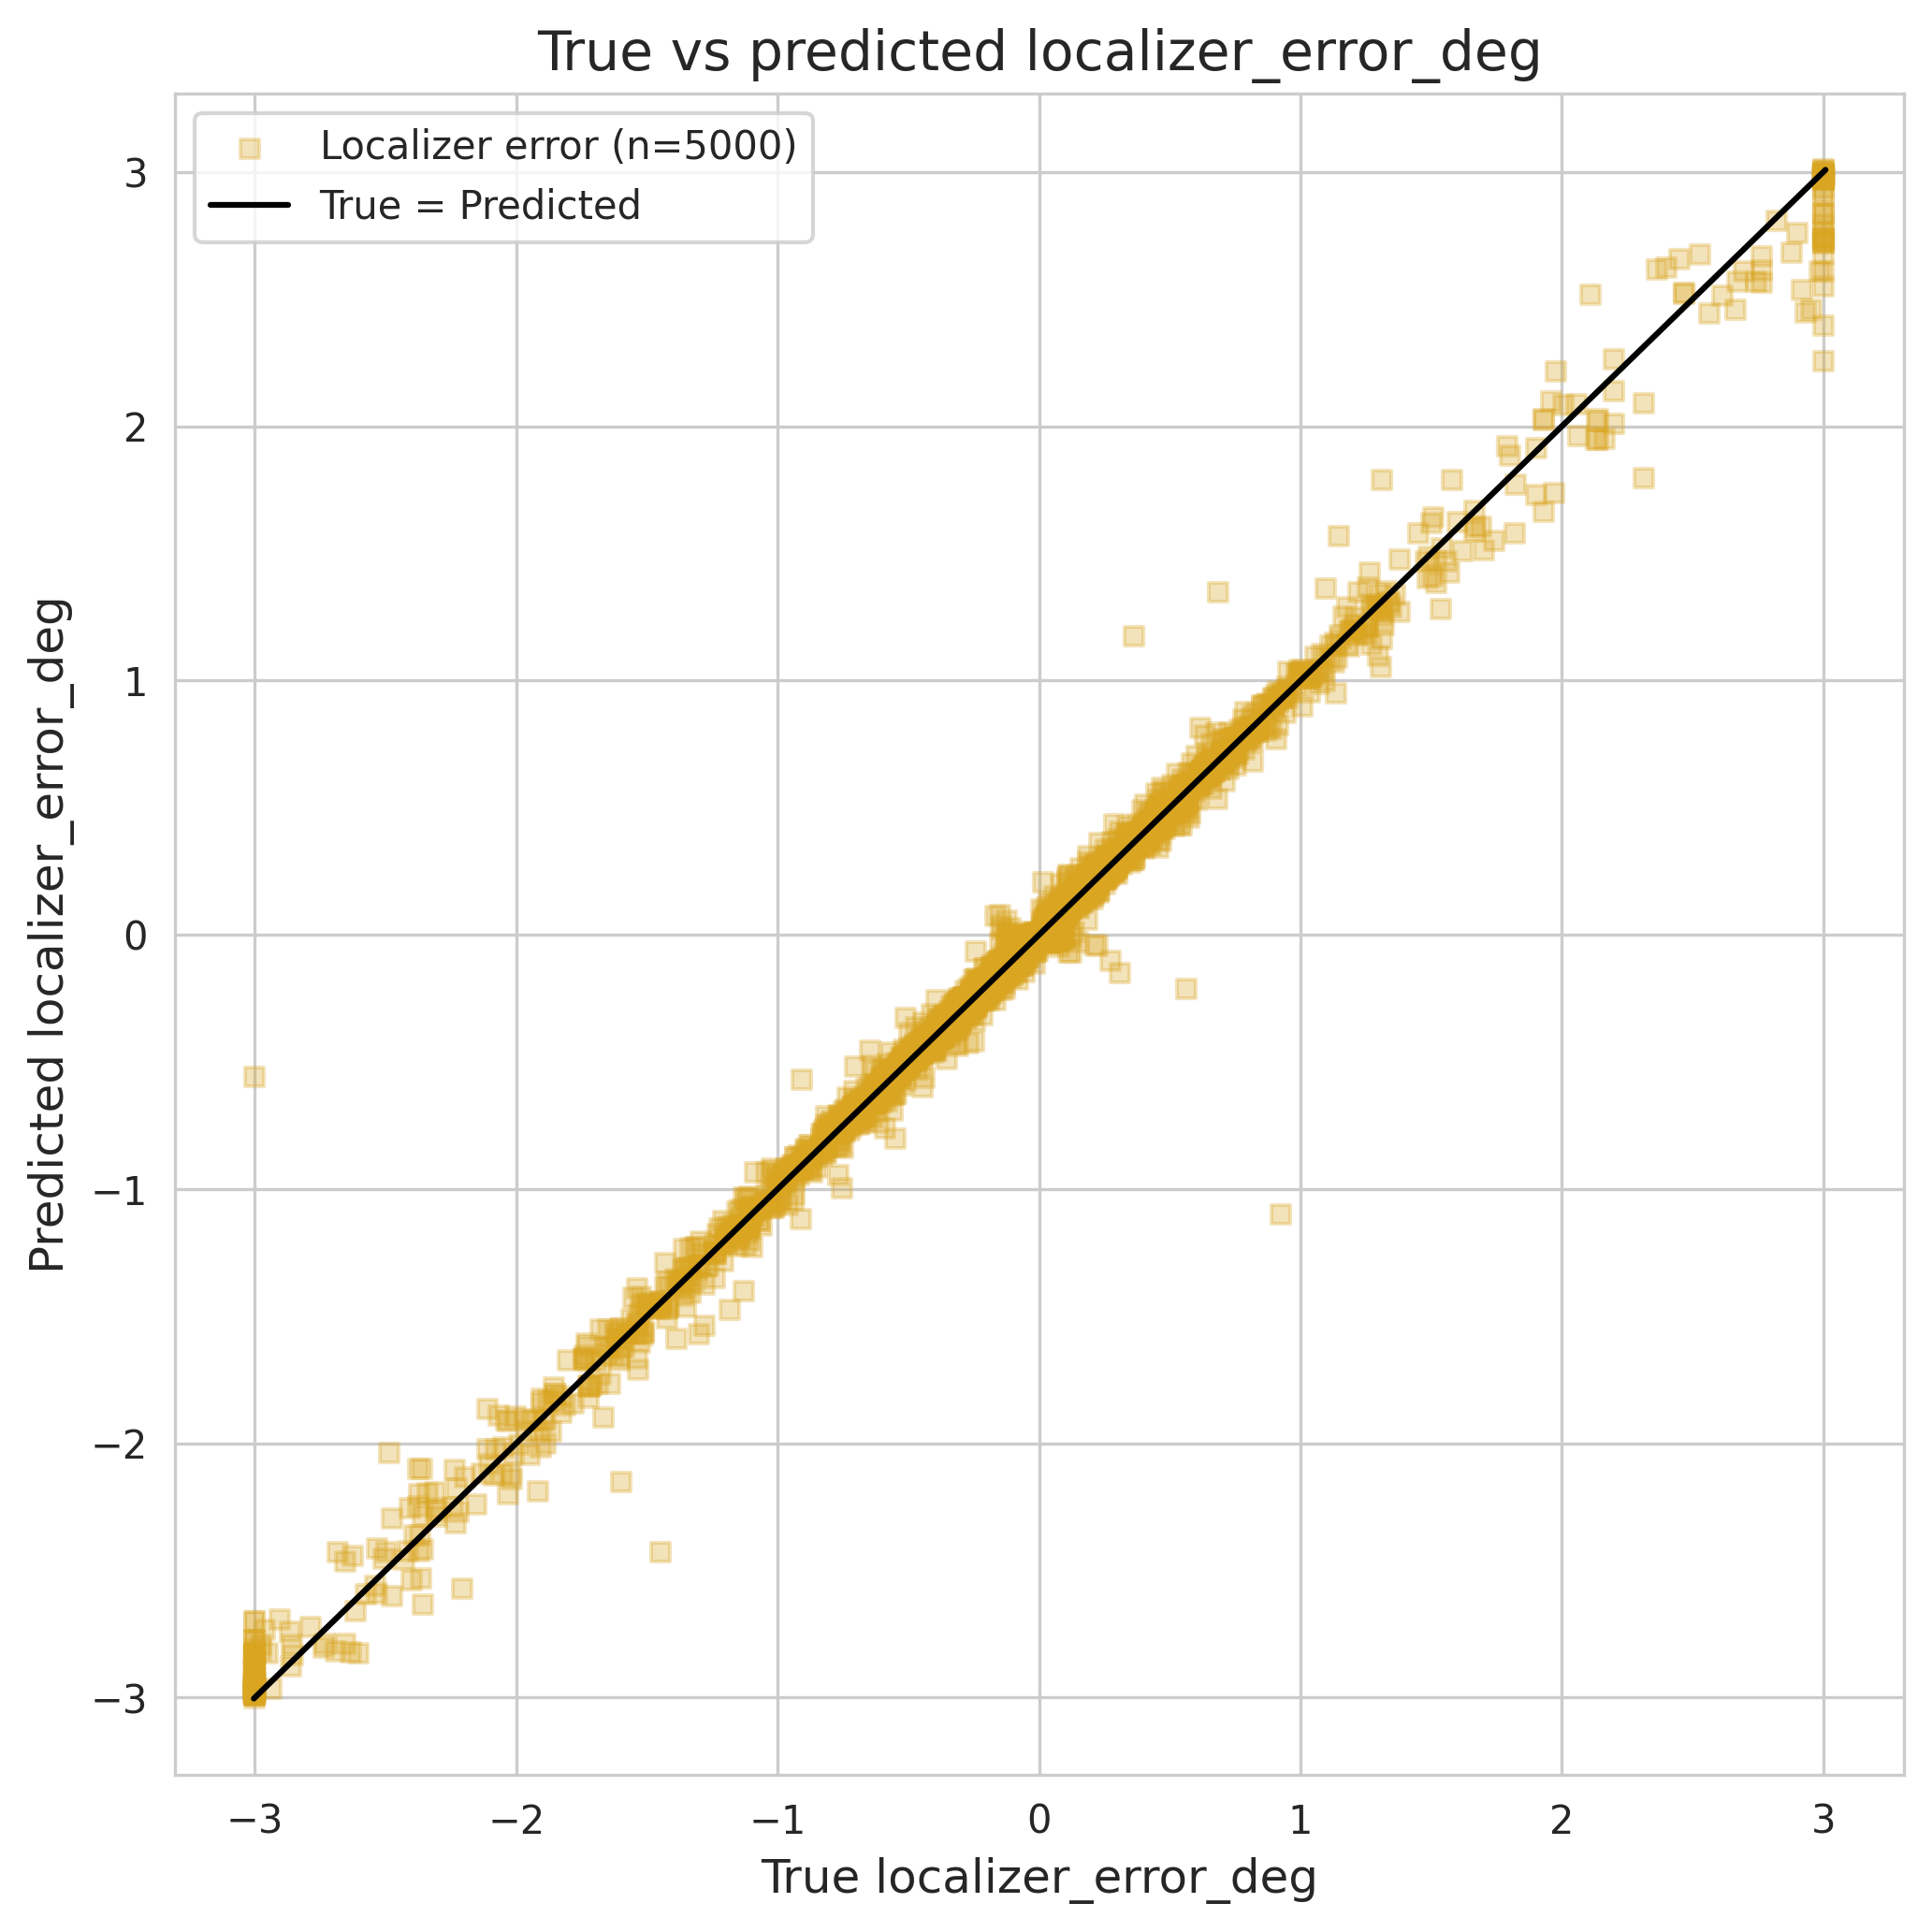
\includegraphics[width=\linewidth]{scatter_true_vs_pred_localizer_error_deg_lag.png}
		\caption{Localizer}
		\label{fig:sub-local}
	\end{subfigure}
	\begin{subfigure}{0.48\textwidth}
		\centering
		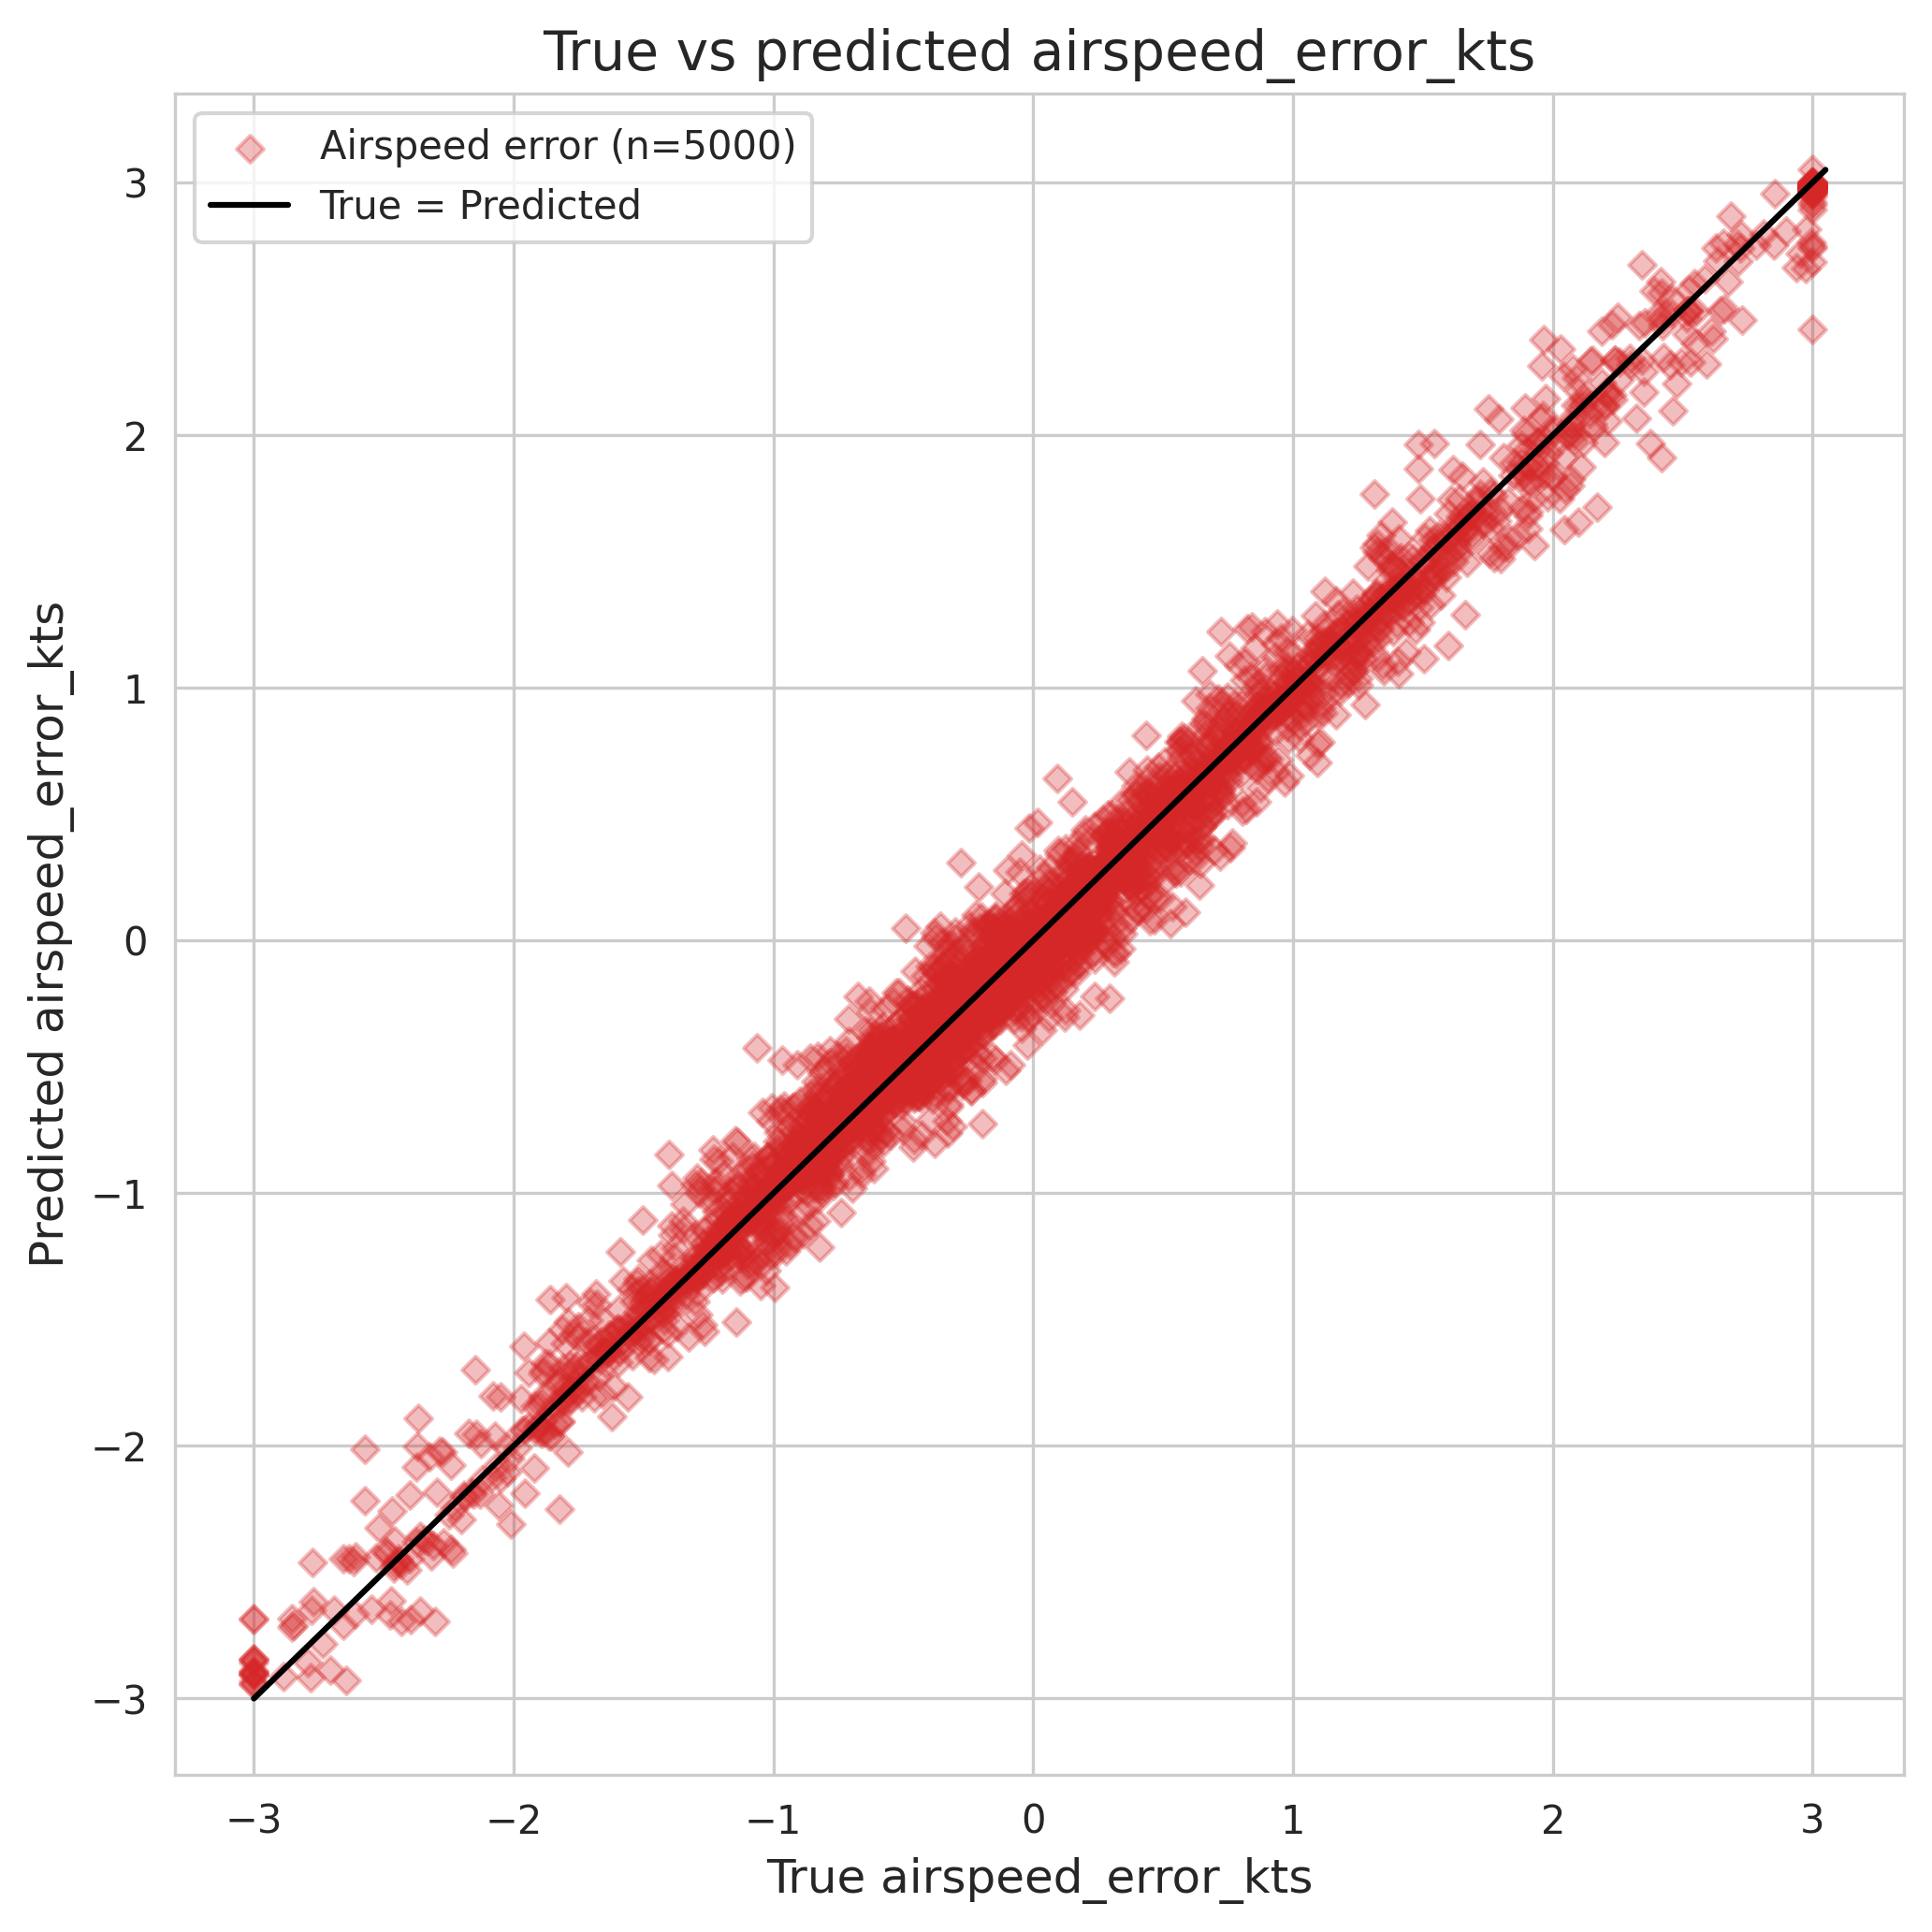
\includegraphics[width=\linewidth]{scatter_true_vs_pred_airspeed_error_kts_lag.png}
		\caption{Airspeed}
		\label{fig:sub-air}
	\end{subfigure}
	\begin{subfigure}{0.48\textwidth}
		\centering
		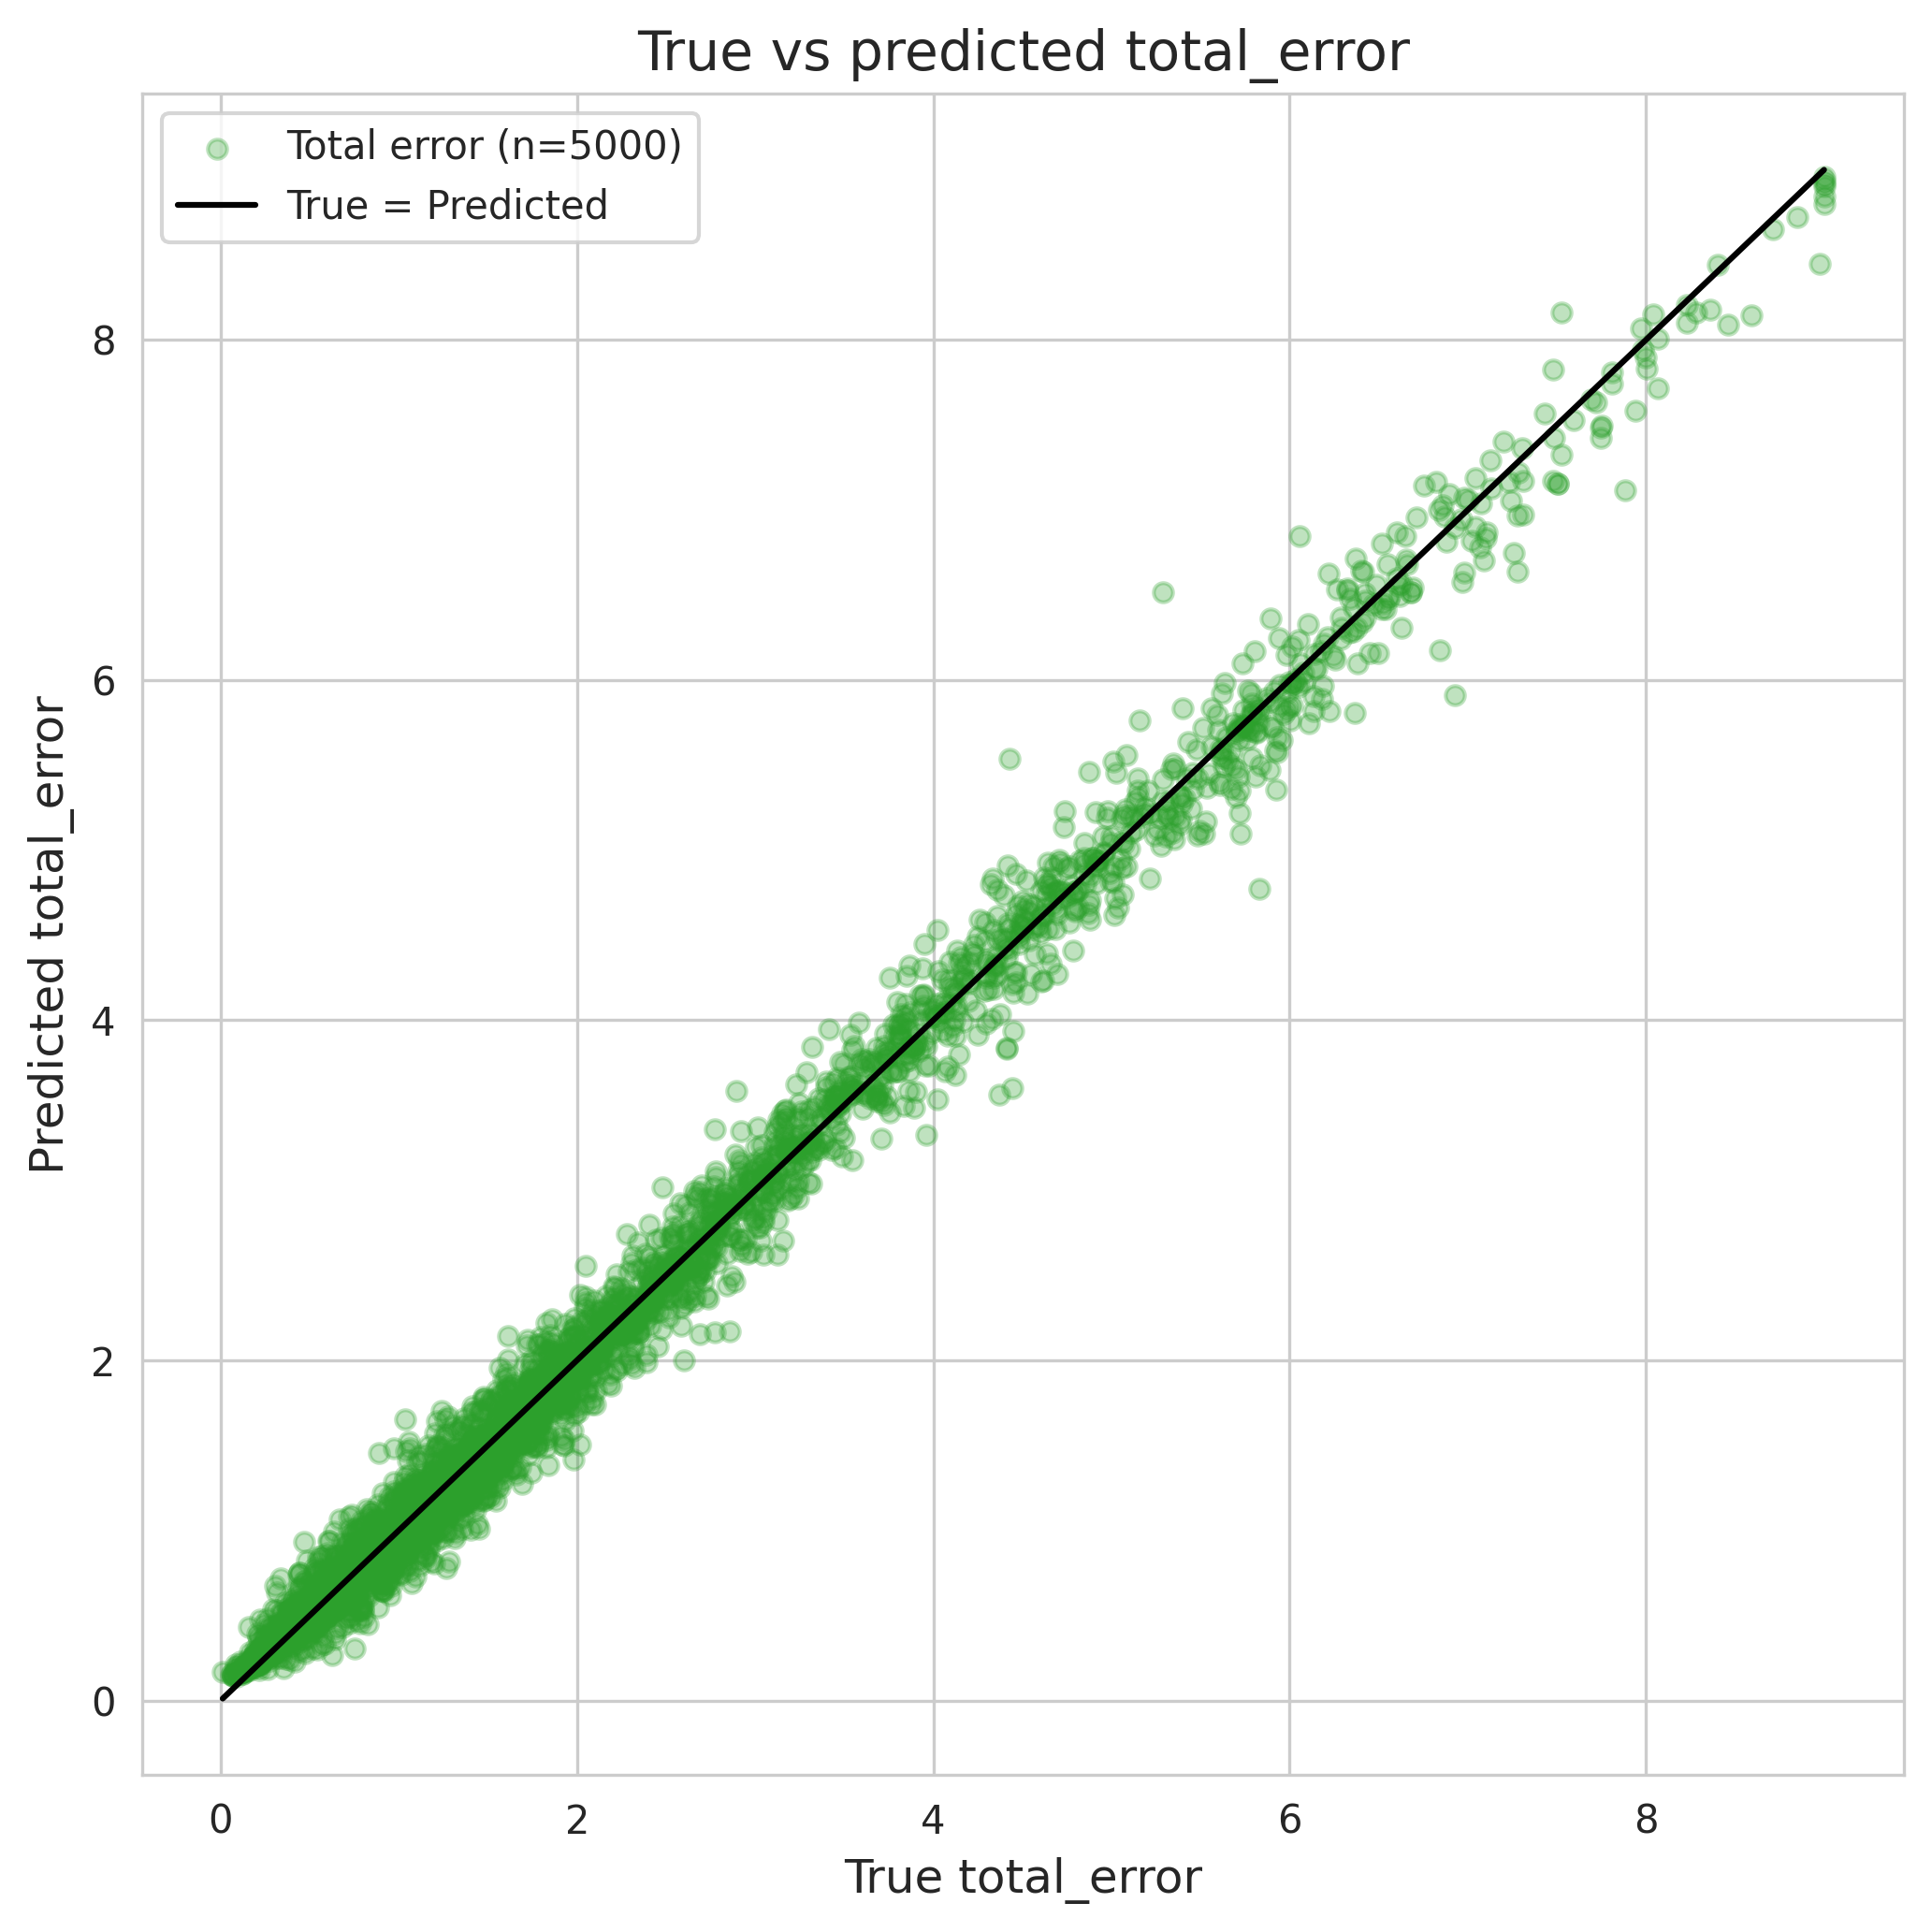
\includegraphics[width=\linewidth]{scatter_true_vs_pred_total_error_lag.png}
		\caption{Total error}
		\label{fig:sub-total}
	\end{subfigure}
	\caption{True–versus–predicted errors (CatBoost generalization on held-out subjects).}
	\label{fig:scatter-all}
\end{figure}

\begin{figure}[htbp]
	\centering
	
\includegraphics[width=\textwidth]{shap_summary_total_error.png}
	\caption{SHAP summary plot for CatBoost in across-time generalization without lagged error inputs.} 
	\label{fig:shap-catboost-temp}
\end{figure}

\begin{figure}[htbp]
	\centering
	
\includegraphics[width=\textwidth]{shap_summary_total_error_lag.png}
	\caption{SHAP summary plot for CatBoost in across-time generalization with lagged error inputs.} 
	\label{fig:shap-catboost-temp-lag}
\end{figure}


\end{document}